\subsection{Fizhi: High-end Atmospheric Physics}
\label{sec:pkg:fizhi}
\begin{rawhtml}
<!-- CMIREDIR:package_fizhi: -->
\end{rawhtml}
%   EPSF.TEX macro file:
%   Written by Tomas Rokicki of Radical Eye Software, 29 Mar 1989.
%   Revised by Don Knuth, 3 Jan 1990.
%   Revised by Tomas Rokicki to accept bounding boxes with no
%      space after the colon, 18 Jul 1990.
%
%   TeX macros to include an Encapsulated PostScript graphic.
%   Works by finding the bounding box comment,
%   calculating the correct scale values, and inserting a vbox
%   of the appropriate size at the current position in the TeX document.
%
%   To use with the center environment of LaTeX, preface the \epsffile
%   call with a \leavevmode.  (LaTeX should probably supply this itself
%   for the center environment.)
%
%   To use, simply say
%   \input epsf           % somewhere early on in your TeX file
%   \epsfbox{filename.ps} % where you want to insert a vbox for a figure
%
%   Alternatively, you can type
%
%   \epsfbox[0 0 30 50]{filename.ps} % to supply your own BB
%
%   which will not read in the file, and will instead use the bounding
%   box you specify.
%
%   The effect will be to typeset the figure as a TeX box, at the
%   point of your \epsfbox command. By default, the graphic will have its
%   `natural' width (namely the width of its bounding box, as described
%   in filename.ps). The TeX box will have depth zero.
%
%   You can enlarge or reduce the figure by saying
%     \epsfxsize=<dimen> \epsfbox{filename.ps}
%   (or
%     \epsfysize=<dimen> \epsfbox{filename.ps})
%   instead. Then the width of the TeX box will be \epsfxsize and its
%   height will be scaled proportionately (or the height will be
%   \epsfysize and its width will be scaled proportiontally).  The
%   width (and height) is restored to zero after each use.
%
%   A more general facility for sizing is available by defining the
%   \epsfsize macro.    Normally you can redefine this macro
%   to do almost anything.  The first parameter is the natural x size of
%   the PostScript graphic, the second parameter is the natural y size
%   of the PostScript graphic.  It must return the xsize to use, or 0 if
%   natural scaling is to be used.  Common uses include:
%
%      \epsfxsize  % just leave the old value alone
%      0pt         % use the natural sizes
%      #1          % use the natural sizes
%      \hsize      % scale to full width
%      0.5#1       % scale to 50% of natural size
%      \ifnum#1>\hsize\hsize\else#1\fi  % smaller of natural, hsize
%
%   If you want TeX to report the size of the figure (as a message
%   on your terminal when it processes each figure), say `\epsfverbosetrue'.
%
\newread\epsffilein    % file to \read
\newif\ifepsffileok    % continue looking for the bounding box?
\newif\ifepsfbbfound   % success?
\newif\ifepsfverbose   % report what you're making?
\newdimen\epsfxsize    % horizontal size after scaling
\newdimen\epsfysize    % vertical size after scaling
\newdimen\epsftsize    % horizontal size before scaling
\newdimen\epsfrsize    % vertical size before scaling
\newdimen\epsftmp      % register for arithmetic manipulation
\newdimen\pspoints     % conversion factor
%
\pspoints=1bp          % Adobe points are `big'
\epsfxsize=0pt         % Default value, means `use natural size'
\epsfysize=0pt         % ditto
%
\def\epsfbox#1{\global\def\epsfllx{72}\global\def\epsflly{72}%
   \global\def\epsfurx{540}\global\def\epsfury{720}%
   \def\lbracket{[}\def\testit{#1}\ifx\testit\lbracket
   \let\next=\epsfgetlitbb\else\let\next=\epsfnormal\fi\next{#1}}%
%
\def\epsfgetlitbb#1#2 #3 #4 #5]#6{\epsfgrab #2 #3 #4 #5 .\\%
   \epsfsetgraph{#6}}%
%
\def\epsfnormal#1{\epsfgetbb{#1}\epsfsetgraph{#1}}%
%
\def\epsfgetbb#1{%
%
%   The first thing we need to do is to open the
%   PostScript file, if possible.
%
\openin\epsffilein=#1
\ifeof\epsffilein\errmessage{I couldn't open #1, will ignore it}\else
%
%   Okay, we got it. Now we'll scan lines until we find one that doesn't
%   start with %. We're looking for the bounding box comment.
%
   {\epsffileoktrue \chardef\other=12
    \def\do##1{\catcode`##1=\other}\dospecials \catcode`\ =10
    \loop
       \read\epsffilein to \epsffileline
       \ifeof\epsffilein\epsffileokfalse\else
%
%   We check to see if the first character is a % sign;
%   if not, we stop reading (unless the line was entirely blank);
%   if so, we look further and stop only if the line begins with
%   `%%BoundingBox:'.
%
          \expandafter\epsfaux\epsffileline:. \\%
       \fi
   \ifepsffileok\repeat
   \ifepsfbbfound\else
    \ifepsfverbose\message{No bounding box comment in #1; using defaults}\fi\fi
   }\closein\epsffilein\fi}%
%
%   Now we have to calculate the scale and offset values to use.
%   First we compute the natural sizes.
%
\def\epsfclipstring{}% do we clip or not?  If so,
\def\epsfclipon{\def\epsfclipstring{ clip}}%
\def\epsfclipoff{\def\epsfclipstring{}}%
%
\def\epsfsetgraph#1{%
   \epsfrsize=\epsfury\pspoints
   \advance\epsfrsize by-\epsflly\pspoints
   \epsftsize=\epsfurx\pspoints
   \advance\epsftsize by-\epsfllx\pspoints
%
%   If `epsfxsize' is 0, we default to the natural size of the picture.
%   Otherwise we scale the graph to be \epsfxsize wide.
%
   \epsfxsize\epsfsize\epsftsize\epsfrsize
   \ifnum\epsfxsize=0 \ifnum\epsfysize=0
      \epsfxsize=\epsftsize \epsfysize=\epsfrsize
      \epsfrsize=0pt
%
%   We have a sticky problem here:  TeX doesn't do floating point arithmetic!
%   Our goal is to compute y = rx/t. The following loop does this reasonably
%   fast, with an error of at most about 16 sp (about 1/4000 pt).
% 
     \else\epsftmp=\epsftsize \divide\epsftmp\epsfrsize
       \epsfxsize=\epsfysize \multiply\epsfxsize\epsftmp
       \multiply\epsftmp\epsfrsize \advance\epsftsize-\epsftmp
       \epsftmp=\epsfysize
       \loop \advance\epsftsize\epsftsize \divide\epsftmp 2
       \ifnum\epsftmp>0
          \ifnum\epsftsize<\epsfrsize\else
             \advance\epsftsize-\epsfrsize \advance\epsfxsize\epsftmp \fi
       \repeat
       \epsfrsize=0pt
     \fi
   \else \ifnum\epsfysize=0
     \epsftmp=\epsfrsize \divide\epsftmp\epsftsize
     \epsfysize=\epsfxsize \multiply\epsfysize\epsftmp   
     \multiply\epsftmp\epsftsize \advance\epsfrsize-\epsftmp
     \epsftmp=\epsfxsize
     \loop \advance\epsfrsize\epsfrsize \divide\epsftmp 2
     \ifnum\epsftmp>0
        \ifnum\epsfrsize<\epsftsize\else
           \advance\epsfrsize-\epsftsize \advance\epsfysize\epsftmp \fi
     \repeat
     \epsfrsize=0pt
    \else
     \epsfrsize=\epsfysize
    \fi
   \fi
%
%  Finally, we make the vbox and stick in a \special that dvips can parse.
%
   \ifepsfverbose\message{#1: width=\the\epsfxsize, height=\the\epsfysize}\fi
   \epsftmp=10\epsfxsize \divide\epsftmp\pspoints
   \vbox to\epsfysize{\vfil\hbox to\epsfxsize{%
      \ifnum\epsfrsize=0\relax
        \special{PSfile=#1 llx=\epsfllx\space lly=\epsflly\space
            urx=\epsfurx\space ury=\epsfury\space rwi=\number\epsftmp
            \epsfclipstring}%
      \else
        \epsfrsize=10\epsfysize \divide\epsfrsize\pspoints
        \special{PSfile=#1 llx=\epsfllx\space lly=\epsflly\space
            urx=\epsfurx\space ury=\epsfury\space rwi=\number\epsftmp\space
            rhi=\number\epsfrsize \epsfclipstring}%
      \fi
      \hfil}}%
\global\epsfxsize=0pt\global\epsfysize=0pt}%
%
%   We still need to define the tricky \epsfaux macro. This requires
%   a couple of magic constants for comparison purposes.
%
{\catcode`\%=12 \global\let\epsfpercent=%\global\def\epsfbblit{%BoundingBox}}%
%
%   So we're ready to check for `%BoundingBox:' and to grab the
%   values if they are found.
%
\long\def\epsfaux#1#2:#3\\{\ifx#1\epsfpercent
   \def\testit{#2}\ifx\testit\epsfbblit
      \epsfgrab #3 . . . \\%
      \epsffileokfalse
      \global\epsfbbfoundtrue
   \fi\else\ifx#1\par\else\epsffileokfalse\fi\fi}%
%
%   Here we grab the values and stuff them in the appropriate definitions.
%
\def\epsfempty{}%
\def\epsfgrab #1 #2 #3 #4 #5\\{%
\global\def\epsfllx{#1}\ifx\epsfllx\epsfempty
      \epsfgrab #2 #3 #4 #5 .\\\else
   \global\def\epsflly{#2}%
   \global\def\epsfurx{#3}\global\def\epsfury{#4}\fi}%
%
%   We default the epsfsize macro.
%
\def\epsfsize#1#2{\epsfxsize}
%
%   Finally, another definition for compatibility with older macros.
%
\let\epsffile=\epsfbox



\subsubsection{Introduction}
The fizhi (high-end atmospheric physics) package includes a collection of state-of-the-art
physical parameterizations for atmospheric radiation, cumulus convection, atmospheric
boundary layer turbulence, and land surface processes. The collection of atmospheric
physics parameterizations were originally used together as part of the GEOS-3
(Goddard Earth Observing System-3) GCM developed at the NASA/Goddard Global Modelling
and Assimilation Office (GMAO).

% *************************************************************************
% *************************************************************************
 
\subsubsection{Equations}

Moist Convective Processes:

\paragraph{Sub-grid and Large-scale Convection}
\label{sec:fizhi:mc}

Sub-grid scale cumulus convection is parameterized using the Relaxed Arakawa
Schubert (RAS) scheme of \cite{moorsz:92}, which is a linearized Arakawa Schubert
type scheme.  RAS predicts the mass flux from an ensemble of clouds.  Each subensemble is identified
by its entrainment rate and level of neutral bouyancy which are determined by the grid-scale properties.

The thermodynamic variables that are used in RAS to describe the grid scale vertical profile are
the dry static energy, $s=c_pT +gz$, and the moist static energy, $h=c_p T + gz + Lq$. 
The conceptual model behind RAS depicts each subensemble as a rising plume cloud, entraining 
mass from the environment during ascent, and detraining all cloud air at the level of neutral 
buoyancy. RAS assumes that the normalized cloud mass flux, $\eta$, normalized by the cloud base 
mass flux, is a linear function of height, expressed as:
\[
\pp{\eta(z)}{z} = \lambda \hspace{0.4cm}or\hspace{0.4cm} \pp{\eta(P^{\kappa})}{P^{\kappa}} = 
-{c_p \over {g}}\theta\lambda
\]
where we have used the hydrostatic equation written in the form:
\[
\pp{z}{P^{\kappa}} = -{c_p \over {g}}\theta
\]

The entrainment parameter, $\lambda$, characterizes a particular subensemble based on its
detrainment level, and is obtained by assuming that the level of detrainment is the level of neutral
buoyancy, ie., the level at which the moist static energy of the cloud, $h_c$, is equal 
to the saturation moist static energy of the environment, $h^*$.  Following \cite{moorsz:92},
$\lambda$ may be written as
\[
\lambda = { {h_B - h^*_D} \over { {c_p \over g} {\int_{P_D}^{P_B}\theta(h^*_D-h)dP^{\kappa}}} } ,
\]

where the subscript $B$ refers to cloud base, and the subscript $D$ refers to the detrainment level.


The convective instability is measured in terms of the cloud work function $A$, defined as the
rate of change of cumulus kinetic energy. The cloud work function is 
related to the buoyancy, or the difference
between the moist static energy in the cloud and in the environment:
\[
A = \int_{P_D}^{P_B} { {\eta \over {1 + \gamma} } 
\left[ {{h_c-h^*} \over {P^{\kappa}}} \right] dP^{\kappa}}
\]

where $\gamma$ is ${L \over {c_p}}\pp{q^*}{T}$ obtained from the Claussius Clapeyron equation,
and the subscript $c$ refers to the value inside the cloud.


To determine the cloud base mass flux, the rate of change of $A$ in time {\em due to dissipation by 
the clouds} is assumed to approximately balance the rate of change of $A$ {\em due to the generation 
by the large scale}. This is the quasi-equilibrium assumption, and results in an expression for $m_B$:
\[
m_B = {{- \left.{dA \over dt} \right|_{ls}} \over K}
\]

where $K$ is the cloud kernel, defined as the rate of change of the cloud work function per
unit cloud base mass flux, and is currently obtained by analytically differentiating the 
expression for $A$ in time.
The rate of change of $A$ due to the generation by the large scale can be written as the
difference between the current $A(t+\Delta t)$ and its equillibrated value after the previous 
convective time step 
$A(t)$, divided by the time step. $A(t)$ is approximated as some critical $A_{crit}$,
computed by Lord (1982) from $in situ$ observations.


The predicted convective mass fluxes are used to solve grid-scale temperature
and moisture budget equations to determine the impact of convection on the large scale fields of
temperature (through latent heating and compensating subsidence) and moisture (through
precipitation and detrainment):
\[
\left.{\pp{\theta}{t}}\right|_{c} = \alpha { m_B \over {c_p P^{\kappa}}} \eta \pp{s}{p}
\]
and
\[
\left.{\pp{q}{t}}\right|_{c} = \alpha { m_B \over {L}} \eta (\pp{h}{p}-\pp{s}{p})
\]
where $\theta = {T \over P^{\kappa}}$, $P = (p/p_0)$, and $\alpha$ is the relaxation parameter.

As an approximation to a full interaction between the different allowable subensembles,
many clouds are simulated frequently, each modifying the large scale environment some fraction
$\alpha$ of the total adjustment. The parameterization thereby ``relaxes'' the large scale environment
towards equillibrium.  

In addition to the RAS cumulus convection scheme, the fizhi package employs a
Kessler-type scheme for the re-evaporation of falling rain (\cite{sudm:88}), which
correspondingly adjusts the temperature assuming $h$ is conserved. RAS in its current
formulation assumes that all cloud water is deposited into the detrainment level as rain.
All of the rain is available for re-evaporation, which begins in the level below detrainment. 
The scheme accounts for some microphysics such as
the rainfall intensity, the drop size distribution, as well as the temperature, 
pressure and relative humidity of the surrounding air.  The fraction of the moisture deficit 
in any model layer into which the rain may re-evaporate is controlled by a free parameter,
which allows for a relatively efficient re-evaporation of liquid precipitate and larger rainout
for frozen precipitation.

Due to the increased vertical resolution near the surface, the lowest model 
layers are averaged to provide a 50 mb thick sub-cloud layer for RAS.  Each time RAS is
invoked (every ten simulated minutes), 
a number of randomly chosen subensembles are checked for the possibility 
of convection, from just above cloud base to 10 mb.  

Supersaturation or large-scale precipitation is initiated in the fizhi package whenever 
the relative humidity in any grid-box exceeds a critical value, currently 100 \%.
The large-scale precipitation re-evaporates during descent to partially saturate 
lower layers in a process identical to the re-evaporation of convective rain. 

 
\paragraph{Cloud Formation}
\label{sec:fizhi:clouds}

Convective and large-scale cloud fractons which are used for cloud-radiative interactions are determined
diagnostically as part of the cumulus and large-scale parameterizations.
Convective cloud fractions produced by RAS are proportional to the 
detrained liquid water amount given by

\[
F_{RAS} = \min\left[ {l_{RAS}\over l_c}, 1.0 \right]
\]

where $l_c$ is an assigned critical value equal to $1.25$ g/kg.
A memory is associated with convective clouds defined by:

\[
F_{RAS}^n = \min\left[ F_{RAS} + (1-{\Delta t_{RAS}\over\tau})F_{RAS}^{n-1}, 1.0 \right]
\]

where $F_{RAS}$ is the instantanious cloud fraction and $F_{RAS}^{n-1}$ is the cloud fraction
from the previous RAS timestep.  The memory coefficient is computed using a RAS cloud timescale,
$\tau$, equal to 1 hour.  RAS cloud fractions are cleared when they fall below 5 \%.

Large-scale cloudiness is defined, following Slingo and Ritter (1985), as a function of relative
humidity:

\[
F_{LS} = \min\left[ { \left( {RH-RH_c \over 1-RH_c} \right) }^2, 1.0 \right]
\]

where

\bqa
RH_c & = & 1-s(1-s)(2-\sqrt{3}+2\sqrt{3} \, s)r \nonumber \\
   s & = & p/p_{surf} \nonumber \\
   r & = & \left( {1.0-RH_{min} \over \alpha} \right) \nonumber \\
RH_{min} & = & 0.75 \nonumber \\
\alpha & = & 0.573285 \nonumber  .
\eqa

These cloud fractions are suppressed, however, in regions where the convective
sub-cloud layer is conditionally unstable.  The functional form of $RH_c$ is shown in
Figure (\ref{fig.rhcrit}).

\begin{figure*}[htbp]
  \vspace{0.4in}
  \centerline{  \epsfysize=4.0in  \epsfbox{part6/rhcrit.ps}}
  \vspace{0.4in}
  \caption  [Critical Relative Humidity for Clouds.]
            {Critical Relative Humidity for Clouds.}
  \label{fig.rhcrit}
\end{figure*}

The total cloud fraction in a grid box is determined by the larger of the two cloud fractions:

\[
F_{CLD} = \max \left[ F_{RAS},F_{LS} \right] .
\]

Finally, cloud fractions are time-averaged between calls to the radiation packages.


Radiation:

The parameterization of radiative heating in the fizhi package includes effects 
from both shortwave and longwave processes.
Radiative fluxes are calculated at each
model edge-level in both up and down directions.
The heating rates/cooling rates are then obtained 
from the vertical divergence of the net radiative fluxes.

The net flux is
\[
F = F^\uparrow - F^\downarrow
\]
where $F$ is the net flux, $F^\uparrow$ is the upward flux and $F^\downarrow$ is
the downward flux.

The heating rate due to the divergence of the radiative flux is given by
\[
\pp{\rho c_p T}{t} = - \pp{F}{z}
\]
or
\[
\pp{T}{t} = \frac{g}{c_p \pi} \pp{F}{\sigma}
\]
where $g$ is the accelation due to gravity
and $c_p$ is the heat capacity of air at constant pressure.
  
The time tendency for Longwave
Radiation is updated every 3 hours.  The time tendency for Shortwave Radiation is updated once
every three hours assuming a normalized incident solar radiation, and subsequently modified at
every model time step by the true incident radiation.  
The solar constant value used in the package is equal to 1365 $W/m^2$
and a $CO_2$ mixing ratio of 330 ppm. 
For the ozone mixing ratio, monthly mean zonally averaged 
climatological values specified as a function
of latitude and height (\cite{rosen:87}) are linearly interpolated to the current time.


\paragraph{Shortwave Radiation}

The shortwave radiation package used in the package computes solar radiative 
heating due to the absoption by water vapor, ozone, carbon dioxide, oxygen,
clouds, and aerosols and due to the
scattering by clouds, aerosols, and gases.
The shortwave radiative processes are described by 
\cite{chou:90,chou:92}. This shortwave package
uses the Delta-Eddington approximation to compute the
bulk scattering properties of a single layer following King and Harshvardhan (JAS, 1986).
The transmittance and reflectance of diffuse radiation
follow the procedures of Sagan and Pollock (JGR, 1967) and \cite{lhans:74}.

Highly accurate heating rate calculations are obtained through the use
of an optimal grouping strategy of spectral bands.  By grouping the UV and visible regions
as indicated in Table \ref{tab:fizhi:solar2}, the Rayleigh scattering and the ozone absorption of solar radiation
can be accurately computed in the ultraviolet region and the photosynthetically
active radiation (PAR) region.
The computation of solar flux in the infrared region is performed with a broadband
parameterization using the spectrum regions shown in Table \ref{tab:fizhi:solar1}.
The solar radiation algorithm used in the fizhi package can be applied not only for climate studies but
also for studies on the photolysis in the upper atmosphere and the photosynthesis in the biosphere.

\begin{table}[htb]
\begin{center}
{\bf UV and Visible Spectral Regions} \\
\vspace{0.1in}
\begin{tabular}{|c|c|c|} 
\hline
Region & Band & Wavelength (micron) \\ \hline
\hline
UV-C   &  1.  &  .175 - .225  \\
       &  2.  &  .225 - .245  \\
       &      &  .260 - .280  \\
       &  3.  &  .245 - .260  \\ \hline
UV-B   &  4.  &  .280 - .295  \\
       &  5.  &  .295 - .310  \\
       &  6.  &  .310 - .320  \\ \hline
UV-A   &  7.  &  .320 - .400  \\ \hline
PAR    &  8.  &  .400 - .700  \\
\hline
\end{tabular}
\end{center}
\caption{UV and Visible Spectral Regions used in shortwave radiation package.}
\label{tab:fizhi:solar2}
\end{table}

\begin{table}[htb]
\begin{center}
{\bf Infrared Spectral Regions} \\
\vspace{0.1in}
\begin{tabular}{|c|c|c|} 
\hline
Band & Wavenumber(cm$^{-1}$) & Wavelength (micron) \\ \hline
\hline
1  &    1000-4400    &    2.27-10.0 \\
2  &    4400-8200    &    1.22-2.27 \\
3  &    8200-14300   &    0.70-1.22 \\
\hline
\end{tabular}
\end{center}
\caption{Infrared Spectral Regions used in shortwave radiation package.}
\label{tab:fizhi:solar1}
\end{table}

Within the shortwave radiation package, 
both ice and liquid cloud particles are allowed to co-exist in any of the model layers. 
Two sets of cloud parameters are used, one for ice paticles and the other for liquid particles.
Cloud parameters are defined as the cloud optical thickness and the effective cloud particle size.
In the fizhi package, the effective radius for water droplets is given as 10 microns,
while 65 microns is used for ice particles.  The absorption due to aerosols is currently
set to zero.

To simplify calculations in a cloudy atmosphere, clouds are
grouped into low ($p>700$ mb), middle (700 mb $\ge p > 400$ mb), and high ($p < 400$ mb) cloud regions. 
Within each of the three regions, clouds are assumed maximally
overlapped, and the cloud cover of the group is the maximum
cloud cover of all the layers in the group.  The optical thickness
of a given layer is then scaled for both the direct (as a function of the
solar zenith angle) and diffuse beam radiation 
so that the grouped layer reflectance is the same as the original reflectance.
The solar flux is computed for each of eight cloud realizations possible within this
low/middle/high classification, and appropriately averaged to produce the net solar flux.

\paragraph{Longwave Radiation}

The longwave radiation package used in the fizhi package is thoroughly described by \cite{chsz:94}.
As described in that document, IR fluxes are computed due to absorption by water vapor, carbon
dioxide, and ozone.  The spectral bands together with their absorbers and parameterization methods,
configured for the fizhi package, are shown in Table \ref{tab:fizhi:longwave}.


\begin{table}[htb]
\begin{center}
{\bf IR Spectral Bands} \\
\vspace{0.1in}
\begin{tabular}{|c|c|l|c| } 
\hline
Band & Spectral Range (cm$^{-1}$) & Absorber & Method \\ \hline
\hline
1   & 0-340      & H$_2$O line      & T \\ \hline
2   & 340-540    & H$_2$O line      & T \\ \hline
3a  & 540-620    & H$_2$O line      & K \\ 
3b  & 620-720    & H$_2$O continuum & S \\ 
3b  & 720-800    & CO$_2$           & T \\ \hline 
4   & 800-980    & H$_2$O line      & K \\ 
    &            & H$_2$O continuum & S \\ \hline 
    &            & H$_2$O line      & K \\ 
5   & 980-1100   & H$_2$O continuum & S \\ 
    &            & O$_3$            & T \\ \hline 
6   & 1100-1380  & H$_2$O line      & K \\ 
    &            & H$_2$O continuum & S \\ \hline
7   & 1380-1900  & H$_2$O line      & T \\ \hline 
8   & 1900-3000  & H$_2$O line      & K \\ \hline 
\hline
\multicolumn{4}{|l|}{ \quad K: {\em k}-distribution method with linear pressure scaling } \\
\multicolumn{4}{|l|}{ \quad T: Table look-up with temperature and pressure scaling } \\
\multicolumn{4}{|l|}{ \quad S: One-parameter temperature scaling } \\
\hline
\end{tabular}
\end{center}
\vspace{0.1in}
\caption{IR Spectral Bands, Absorbers, and Parameterization Method (from \cite{chsz:94})}
\label{tab:fizhi:longwave}
\end{table}


The longwave radiation package accurately computes cooling rates for the middle and 
lower atmosphere from 0.01 mb to the surface.  Errors are $<$ 0.4 C day$^{-1}$ in cooling
rates and $<$ 1\% in fluxes.  From Chou and Suarez, it is estimated that the total effect of 
neglecting all minor absorption bands and the effects of minor infrared absorbers such as
nitrous oxide (N$_2$O), methane (CH$_4$), and the chlorofluorocarbons (CFCs), is an underestimate
of $\approx$ 5 W/m$^2$ in the downward flux at the surface and an overestimate of $\approx$ 3 W/m$^2$
in the upward flux at the top of the atmosphere.

Similar to the procedure used in the shortwave radiation package, clouds are grouped into
three regions catagorized as low/middle/high.
The net clear line-of-site probability $(P)$ between any two levels, $p_1$ and $p_2 \quad (p_2 > p_1)$,  
assuming randomly overlapped cloud groups, is simply the product of the probabilities within each group:

\[ P_{net} = P_{low} \times P_{mid} \times P_{hi} . \]

Since all clouds within a group are assumed maximally overlapped, the clear line-of-site probability within
a group is given by:

\[ P_{group} = 1 - F_{max} , \]

where $F_{max}$ is the maximum cloud fraction encountered between $p_1$ and $p_2$ within that group.
For groups and/or levels outside the range of $p_1$ and $p_2$, a clear line-of-site probability equal to 1 is
assigned.


\paragraph{Cloud-Radiation Interaction}
\label{sec:fizhi:radcloud}

The cloud fractions and diagnosed cloud liquid water produced by moist processes 
within the fizhi package are used in the radiation packages to produce cloud-radiative forcing.
The cloud optical thickness associated with large-scale cloudiness is made
proportional to the diagnosed large-scale liquid water, $\ell$, detrained due to super-saturation.
Two values are used corresponding to cloud ice particles and water droplets.
The range of optical thickness for these clouds is given as

\[ 0.0002 \le \tau_{ice} (mb^{-1}) \le 0.002  \quad\mbox{for}\quad  0 \le \ell \le 2 \quad\mbox{mg/kg} , \]
\[ 0.02 \le \tau_{h_2o} (mb^{-1}) \le 0.2  \quad\mbox{for}\quad  0 \le \ell \le 10 \quad\mbox{mg/kg} . \]

The partitioning, $\alpha$,  between ice particles and water droplets is achieved through a linear scaling
in temperature:

\[ 0 \le \alpha \le 1 \quad\mbox{for}\quad  233.15 \le T \le 253.15 . \]

The resulting optical depth associated with large-scale cloudiness is given as

\[ \tau_{LS} = \alpha \tau_{h_2o} + (1-\alpha)\tau_{ice} . \]

The optical thickness associated with sub-grid scale convective clouds produced by RAS is given as

\[ \tau_{RAS} = 0.16 \quad mb^{-1} . \]

The total optical depth in a given model layer is computed as a weighted average between
the large-scale and sub-grid scale optical depths, normalized by the total cloud fraction in the
layer:

\[ \tau = \left( {F_{RAS} \,\,\, \tau_{RAS} + F_{LS} \,\,\, \tau_{LS} \over F_{RAS}+F_{LS} } \right) \Delta p, \]

where $F_{RAS}$ and $F_{LS}$ are the time-averaged cloud fractions associated with RAS and large-scale
processes described in Section \ref{sec:fizhi:clouds}.
The optical thickness for the longwave radiative feedback is assumed to be 75 $\%$ of these values.

The entire Moist Convective Processes Module is called with a frequency of 10 minutes. 
The cloud fraction values are time-averaged over the period between Radiation calls (every 3
hours).  Therefore, in a time-averaged sense, both convective and large-scale 
cloudiness can exist in a given grid-box.  

\paragraph{Turbulence}:

Turbulence is parameterized in the fizhi package to account for its contribution to the
vertical exchange of heat, moisture, and momentum.  
The turbulence scheme is invoked every 30 minutes, and employs a backward-implicit iterative 
time scheme with an internal time step of 5 minutes.
The tendencies of atmospheric state variables due to turbulent diffusion are calculated using
the diffusion equations:

\[
{\pp{u}{t}}_{turb} = {\pp{}{z} }{(- \overline{u^{\prime}w^{\prime}})}
 = {\pp{}{z} }{(K_m \pp{u}{z})}
\]
\[
{\pp{v}{t}}_{turb} = {\pp{}{z} }{(- \overline{v^{\prime}w^{\prime}})}
 = {\pp{}{z} }{(K_m \pp{v}{z})}
\]
\[
{\pp{T}{t}} = P^{\kappa}{\pp{\theta}{t}}_{turb} = 
P^{\kappa}{\pp{}{z} }{(- \overline{w^{\prime}\theta^{\prime}})}
 = P^{\kappa}{\pp{}{z} }{(K_h \pp{\theta_v}{z})}
\]
\[
{\pp{q}{t}}_{turb} = {\pp{}{z} }{(- \overline{w^{\prime}q^{\prime}})}
 = {\pp{}{z} }{(K_h \pp{q}{z})}
\]

Within the atmosphere, the time evolution
of second turbulent moments is explicitly modeled by representing the third moments in terms of 
the first and second moments.  This approach is known as a second-order closure modeling.
To simplify and streamline the computation of the second moments, the level 2.5 assumption
of Mellor and Yamada (1974) and \cite{yam:77} is employed, in which only the turbulent 
kinetic energy (TKE),

\[ {\h}{q^2}={\overline{{u^{\prime}}^2}}+{\overline{{v^{\prime}}^2}}+{\overline{{w^{\prime}}^2}}, \]

is solved prognostically and the other second moments are solved diagnostically.
The prognostic equation for TKE allows the scheme to simulate 
some of the transient and diffusive effects in the turbulence. The TKE budget equation
is solved numerically using an implicit backward computation of the terms linear in $q^2$
and is written:

\[
{\dd{}{t} ({{\h} q^2})} - { \pp{}{z} ({ {5 \over 3} {{\lambda}_1} q { \pp {}{z} 
({\h}q^2)} })} =
{- \overline{{u^{\prime}}{w^{\prime}}} { \pp{U}{z} }} - {\overline{{v^{\prime}}{w^{\prime}}} 
{ \pp{V}{z} }} + {{g \over {\Theta_0}}{\overline{{w^{\prime}}{{{\theta}_v}^{\prime}}}} } 
- { q^3 \over {{\Lambda} _1} }
\]

where $q$ is the turbulent velocity, ${u^{\prime}}$, ${v^{\prime}}$, ${w^{\prime}}$ and 
${{\theta}^{\prime}}$ are the fluctuating parts of the velocity components and potential 
temperature, $U$ and $V$ are the mean velocity components, ${\Theta_0}^{-1}$ is the
coefficient of thermal expansion, and ${{\lambda}_1}$ and ${{\Lambda} _1}$ are constant
multiples of the master length scale, $\ell$, which is designed to be a characteristic measure
of the vertical structure of the turbulent layers.

The first term on the left-hand side represents the time rate of change of TKE, and
the second term is a representation of the triple correlation, or turbulent
transport term. The first three terms on the right-hand side represent the sources of
TKE due to shear and bouyancy, and the last term on the right hand side is the dissipation
of TKE.

In the level 2.5 approach, the vertical fluxes of the scalars $\theta_v$ and $q$ and the
wind components $u$ and $v$ are expressed in terms of the diffusion coefficients $K_h$ and
$K_m$, respectively.  In the statisically realizable level 2.5 turbulence scheme of 
\cite{helflab:88}, these diffusion coefficients are expressed as

\[
K_h 
 = \left\{ \begin{array}{l@{\quad\mbox{for}\quad}l} q \, \ell \, S_H(G_M,G_H) \, & \mbox{decaying turbulence}
\\ { q^2 \over {q_e} } \, \ell \, S_{H}(G_{M_e},G_{H_e}) \, & \mbox{growing turbulence} \end{array} \right.
\]

and

\[
K_m
 = \left\{ \begin{array}{l@{\quad\mbox{for}\quad}l} q \, \ell \, S_M(G_M,G_H) \, & \mbox{decaying turbulence}                
\\ { q^2 \over {q_e} } \, \ell \, S_{M}(G_{M_e},G_{H_e}) \, & \mbox{growing turbulence} \end{array} \right.
\]

where the subscript $e$ refers to the value under conditions of local equillibrium
(obtained from the Level 2.0 Model), $\ell$ is the master length scale related to the 
vertical structure of the atmosphere,
and $S_M$ and $S_H$ are functions of $G_H$ and $G_M$, the dimensionless buoyancy and
wind shear parameters, respectively.
Both $G_H$ and $G_M$, and their equilibrium values $G_{H_e}$ and $G_{M_e}$,
are functions of the Richardson number:

\[
{\bf RI} = { { {g \over \theta_v} \pp {\theta_v}{z} } \over { (\pp{u}{z})^2 + (\pp{v}{z})^2 } }
 =  {  {c_p \pp{\theta_v}{z} \pp{P^ \kappa}{z} } \over { (\pp{u}{z})^2 + (\pp{v}{z})^2 } } .
\]

Negative values indicate unstable buoyancy and shear, small positive values ($<0.2$)
indicate dominantly unstable shear, and large positive values indicate dominantly stable
stratification.

Turbulent eddy diffusion coefficients of momentum, heat and moisture in the surface layer,
which corresponds to the lowest GCM level (see \ref{tab:fizhi:sigma}),
are calculated using stability-dependant functions based on Monin-Obukhov theory:
\[
{K_m} (surface) = C_u \times u_* = C_D W_s
\]
and
\[
{K_h} (surface) =  C_t \times u_* = C_H W_s
\]
where $u_*=C_uW_s$ is the surface friction velocity,
$C_D$ is termed the surface drag coefficient, $C_H$ the heat transfer coefficient, 
and $W_s$ is the magnitude of the surface layer wind.

$C_u$ is the dimensionless exchange coefficient for momentum from the surface layer
similarity functions: 
\[
{C_u} = {u_* \over W_s} = { k \over \psi_{m} }
\]
where k is the Von Karman constant and $\psi_m$ is the surface layer non-dimensional 
wind shear given by
\[
\psi_{m} = {\int_{\zeta_{0}}^{\zeta} {\phi_{m} \over \zeta} d \zeta} .
\]
Here $\zeta$ is the non-dimensional stability parameter, and
$\phi_m$ is the similarity function of $\zeta$ which expresses the stability dependance of
the momentum gradient.  The functional form of $\phi_m$ is specified differently for stable and unstable 
layers.

$C_t$ is the dimensionless exchange coefficient for heat and 
moisture from the surface layer similarity functions:
\[
{C_t} = -{( {\overline{w^{\prime}\theta^{\prime}}}) \over {u_* \Delta \theta }} =
-{( {\overline{w^{\prime}q^{\prime}}}) \over {u_* \Delta q }} =
{ k \over { (\psi_{h} + \psi_{g}) } }
\]
where $\psi_h$ is the surface layer non-dimensional temperature gradient given by
\[
\psi_{h} = {\int_{\zeta_{0}}^{\zeta} {\phi_{h} \over \zeta} d \zeta} .
\]
Here $\phi_h$ is the similarity function of $\zeta$, which expresses the stability dependance of
the temperature and moisture gradients, and is specified differently for stable and unstable
layers according to \cite{helfschu:95}.

$\psi_g$ is the non-dimensional temperature or moisture gradient in the viscous sublayer, 
which is the mosstly laminar region between the surface and the tops of the roughness 
elements, in which temperature and moisture gradients can be quite large.
Based on \cite{yagkad:74}:
\[
\psi_{g} = { 0.55 (Pr^{2/3} - 0.2) \over \nu^{1/2} }
(h_{0}u_{*} - h_{0_{ref}}u_{*_{ref}})^{1/2}
\]
where Pr is the Prandtl number for air, $\nu$ is the molecular viscosity, $z_{0}$ is the 
surface roughness length, and the subscript {\em ref} refers to a reference value.
$h_{0} = 30z_{0}$ with a maximum value over land of 0.01
 
The surface roughness length over oceans is is a function of the surface-stress velocity,
\[
{z_0} = c_1u^3_* + c_2u^2_* + c_3u_* + c_4 + {c_5 \over {u_*}}
\]
where the constants are chosen to interpolate between the reciprocal relation of
\cite{kondo:75} for weak winds, and the piecewise linear relation of \cite{larpond:81}
for moderate to large winds.  Roughness lengths over land are specified
from the climatology of \cite{dorsell:89}.

For an unstable surface layer, the stability functions, chosen to interpolate between the
condition of small values of $\beta$ and the convective limit, are the KEYPS function 
(\cite{pano:73}) for momentum, and its generalization for heat and moisture:  
\[
{\phi_m}^4 - 18 \zeta {\phi_m}^3 = 1 \hspace{1cm} ; \hspace{1cm} 
{\phi_h}^2 - 18 \zeta {\phi_h}^3 = 1 \hspace{1cm} .
\]
The function for heat and moisture assures non-vanishing heat and moisture fluxes as the wind 
speed approaches zero. 

For a stable surface layer, the stability functions are the observationally 
based functions of \cite{clarke:70},  slightly modified for
the momemtum flux:  
\[
{\phi_m} = { { 1 + 5 {{\zeta}_1} } \over { 1 + 0.00794 {{\zeta}_1}
(1+ 5 {{\zeta}_1}) } } \hspace{1cm} ; \hspace{1cm}
{\phi_h} = { { 1 + 5 {{\zeta}_1} } \over { 1 + 0.00794 {\zeta}
(1+ 5 {{\zeta}_1}) } } .
\]
The moisture flux also depends on a specified evapotranspiration
coefficient, set to unity over oceans and dependant on the climatological ground wetness over
land.  

Once all the diffusion coefficients are calculated, the diffusion equations are solved numerically
using an implicit backward operator.

\paragraph{Atmospheric Boundary Layer}

The depth of the atmospheric boundary layer (ABL) is diagnosed by the parameterization as the
level at which the turbulent kinetic energy is reduced to a tenth of its maximum near surface value.
The vertical structure of the ABL is explicitly resolved by the lowest few (3-8) model layers.

\paragraph{Surface Energy Budget}

The ground temperature equation is solved as part of the turbulence package
using a backward implicit time differencing scheme:
\[
C_g\pp{T_g}{t} = R_{sw} - R_{lw} + Q_{ice} - H - LE
\]
where $R_{sw}$ is the net surface downward shortwave radiative flux and $R_{lw}$ is the
net surface upward longwave radiative flux. 

$H$ is the upward sensible heat flux, given by:
\[
{H} =  P^{\kappa}\rho c_{p} C_{H} W_s (\theta_{surface} - \theta_{NLAY})
\hspace{1cm}where: \hspace{.2cm}C_H = C_u C_t
\]
where $\rho$ = the atmospheric density at the surface, $c_{p}$ is the specific
heat of air at constant pressure, and $\theta$ represents the potential temperature
of the surface and of the lowest $\sigma$-level, respectively.
 
The upward latent heat flux, $LE$, is given by
\[
{LE} =  \rho \beta L C_{H} W_s (q_{surface} - q_{NLAY})
\hspace{1cm}where: \hspace{.2cm}C_H = C_u C_t
\]
where $\beta$ is the fraction of the potential evapotranspiration actually evaporated,
L is the latent heat of evaporation, and $q_{surface}$ and $q_{NLAY}$ are the specific
humidity of the surface and of the lowest $\sigma$-level, respectively.

The heat conduction through sea ice, $Q_{ice}$, is given by
\[
{Q_{ice}} = {C_{ti} \over {H_i}} (T_i-T_g)
\]
where $C_{ti}$ is the thermal conductivity of ice, $H_i$ is the ice thickness, assumed to
be $3 \hspace{.1cm} m$ where sea ice is present, $T_i$ is 273 degrees Kelvin, and $T_g$ is the 
surface temperature of the ice.

$C_g$ is the total heat capacity of the ground, obtained by solving a heat diffusion equation
for the penetration of the diurnal cycle into the ground (\cite{black:77}), and is given by:
\[
C_g = \sqrt{ {\lambda C_s \over 2\omega} } = \sqrt{(0.386 + 0.536W + 0.15W^2)2\times10^{-3}
{86400 \over 2 \pi} } \, \, .
\]
Here, the thermal conductivity, $\lambda$, is equal to $2\times10^{-3}$ ${ly\over{ sec}}
{cm \over {^oK}}$,    
the angular velocity of the earth, $\omega$, is written as $86400$ $sec/day$ divided
by $2 \pi$ $radians/  
day$, and the expression for $C_s$, the heat capacity per unit volume at the surface,
is a function of the ground wetness, $W$.

Land Surface Processes:

\paragraph{Surface Type}
The fizhi package surface Types are designated using the Koster-Suarez (\cite{ks:91,ks:92}) 
Land Surface Model (LSM) mosaic philosophy which allows multiple ``tiles'', or multiple surface 
types, in any one grid cell. The Koster-Suarez LSM surface type classifications
are shown in Table \ref{tab:fizhi:surftype}. The surface types and the percent of the grid
cell occupied by any surface type were derived from the surface classification of
\cite{deftow:94}, and information about the location of permanent
ice was obtained from the classifications of \cite{dorsell:89}.
The surface type map for a $1^\circ$ grid is shown in Figure \ref{fig:fizhi:surftype}.
The determination of the land or sea category of surface type was made from NCAR's
10 minute by 10 minute Navy topography 
dataset, which includes information about the percentage of water-cover at any point.
The data were averaged to the model's grid resolutions,
and any grid-box whose averaged water percentage was $\geq 60 \%$ was
defined as a water point. The Land-Water designation was further modified
subjectively to ensure sufficient representation from small but isolated land and water regions.
 
\begin{table}
\begin{center}
{\bf Surface Type Designation} \\
\vspace{0.1in}
\begin{tabular}{ |c|l| }
\hline
Type & Vegetation Designation \\ \hline
\hline
  1 & Broadleaf Evergreen Trees \\ \hline
  2 & Broadleaf Deciduous Trees \\ \hline
  3 & Needleleaf Trees \\ \hline
  4 & Ground Cover \\ \hline   
  5 & Broadleaf Shrubs \\ \hline
  6 & Dwarf Trees (Tundra) \\ \hline
  7 & Bare Soil \\ \hline
  8 & Desert (Bright) \\ \hline
  9 & Glacier \\ \hline
 10 & Desert (Dark) \\ \hline
100 & Ocean \\ \hline
\end{tabular}
\end{center}
\caption{Surface type designations used to compute surface roughness (over land) 
and surface albedo.}
\label{tab:fizhi:surftype}
\end{table}
 
 
\begin{figure*}[htbp]
  \begin{center}
  \rotatebox{270}{\resizebox{90mm}{!}{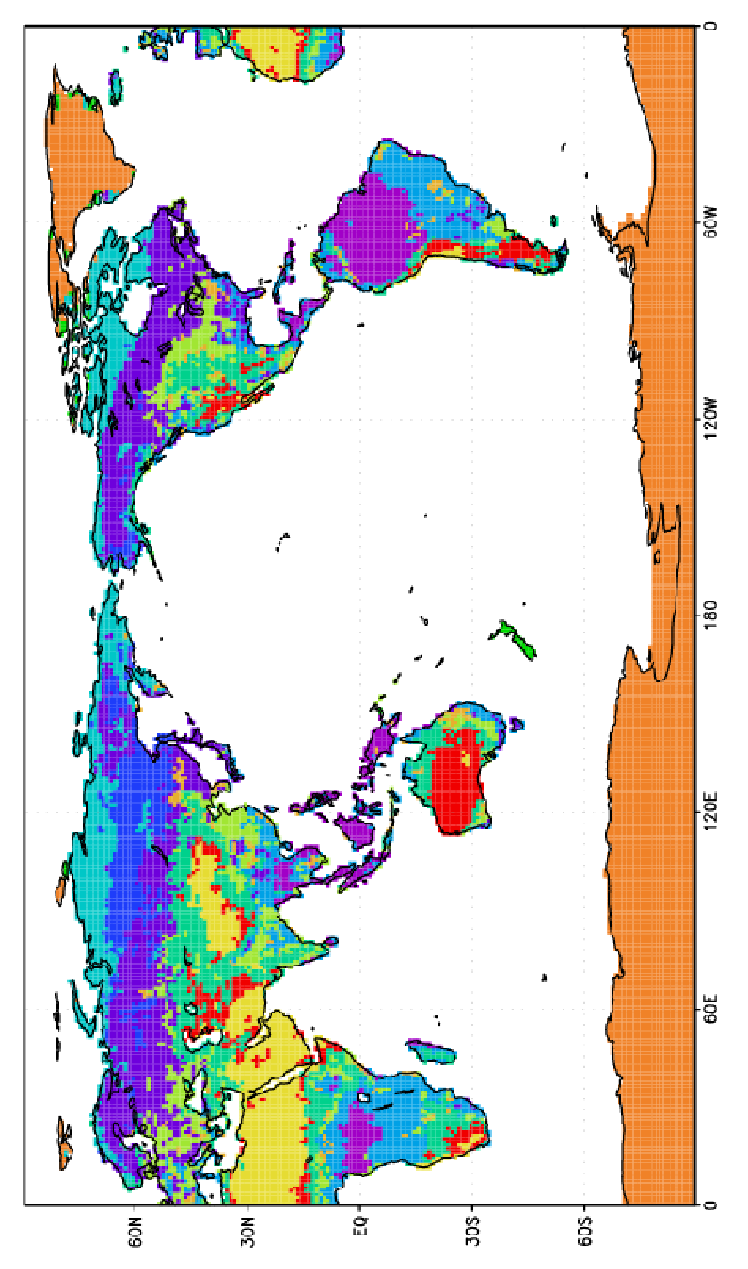
\includegraphics{part6/surftypes.eps}}}
  \rotatebox{270}{\resizebox{100mm}{!}{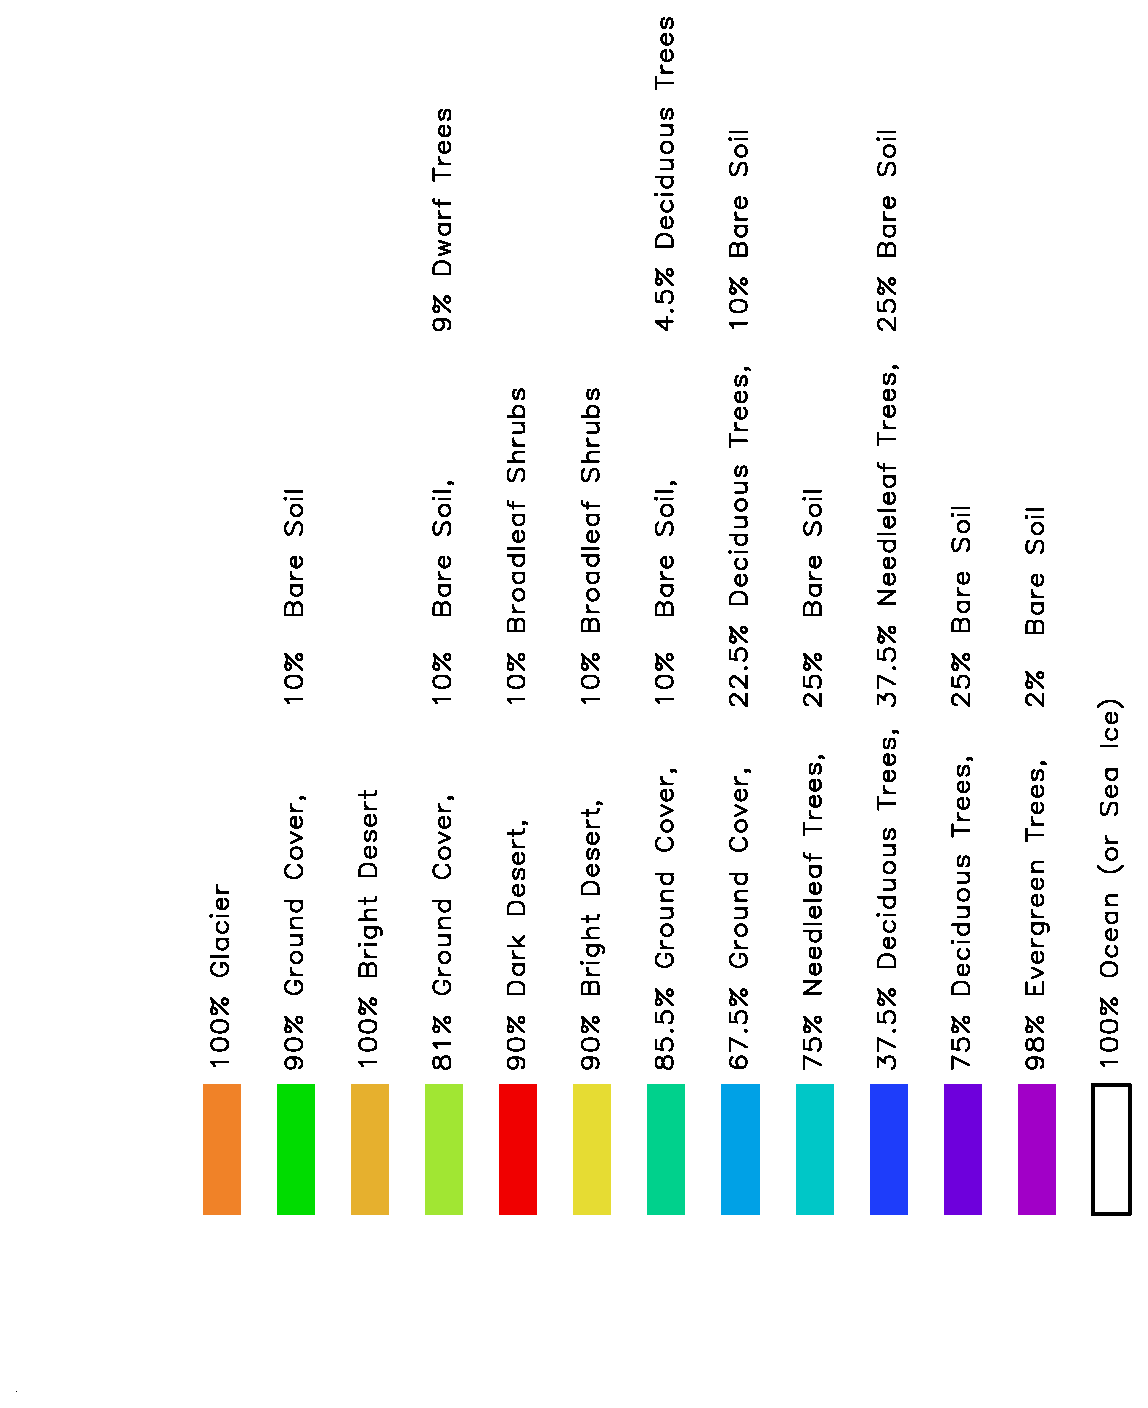
\includegraphics{part6/surftypes.descrip.eps}}}
  \end{center}
  \vspace{0.2in}
  \caption  {Surface Type Combinations at $1^\circ$ resolution.}
  \label{fig:fizhi:surftype}
\end{figure*}

% \rotatebox{270}{\centerline{  \epsfysize=4in  \epsfbox{part6/surftypes.eps}}}
% \rotatebox{270}{\centerline{  \epsfysize=4in  \epsfbox{part6/surftypes.descrip.eps}}}
%\begin{figure*}[htbp]
%  \centerline{  \epsfysize=4in  \epsfbox{part6/surftypes.descrip.ps}}
%  \vspace{0.3in}
%  \caption  {Surface Type Descriptions.}
%  \label{fig:fizhi:surftype.desc}
%\end{figure*}


\paragraph{Surface Roughness}
The surface roughness length over oceans is computed iteratively with the wind
stress by the surface layer parameterization (\cite{helfschu:95}).
It employs an interpolation between the functions of \cite{larpond:81}
for high winds and of \cite{kondo:75} for weak winds.


\paragraph{Albedo}
The surface albedo computation, described in \cite{ks:91},
employs the ``two stream'' approximation used in Sellers' (1987) Simple Biosphere (SiB)
Model which distinguishes between the direct and diffuse albedos in the visible
and in the near infra-red spectral ranges. The albedos are functions of the observed
leaf area index (a description of the relative orientation of the leaves to the
sun), the greenness fraction, the vegetation type, and the solar zenith angle.
Modifications are made to account for the presence of snow, and its depth relative
to the height of the vegetation elements.

\paragraph{Gravity Wave Drag}:

The fizhi package employs the gravity wave drag scheme of \cite{zhouetal:95}).
This scheme is a modified version of Vernekar et al. (1992),
which was based on Alpert et al. (1988) and Helfand et al. (1987).  
In this version, the gravity wave stress at the surface is
based on that derived by Pierrehumbert (1986) and is given by:

\bq
|\vec{\tau}_{sfc}| = {\rho U^3\over{N \ell^*}} \left(F_r^2 \over{1+F_r^2}\right) \, \, ,
\eq

where $F_r = N h /U$ is the Froude number, $N$ is the {\em Brunt - V\"{a}is\"{a}l\"{a}} frequency, $U$ is the 
surface wind speed, $h$ is the standard deviation of the sub-grid scale orography,
and $\ell^*$ is the wavelength of the monochromatic gravity wave in the direction of the low-level wind.
A modification introduced by Zhou et al. allows for the momentum flux to
escape through the top of the model, although this effect is small for the current 70-level model.  
The subgrid scale standard deviation is defined by $h$, and is not allowed to exceed 400 m. 

The effects of using this scheme within a GCM are shown in \cite{taksz:96}.
Experiments using the gravity wave drag parameterization yielded significant and
beneficial impacts on both the time-mean flow and the transient statistics of the
a GCM climatology, and have eliminated most of the worst dynamically driven biases 
in the a GCM simulation. 
An examination of the angular momentum budget during climate runs indicates that the 
resulting gravity wave torque is similar to the data-driven torque produced by a data 
assimilation which was performed without gravity
wave drag.  It was shown that the inclusion of gravity wave drag results in 
large changes in both the mean flow and in eddy fluxes.
The result is a more
accurate simulation of surface stress (through a reduction in the surface wind strength), 
of mountain torque (through a redistribution of mean sea-level pressure), and of momentum
convergence (through a reduction in the flux of westerly momentum by transient flow eddies).  


Boundary Conditions and other Input Data:

Required fields which are not explicitly predicted or diagnosed during model execution must
either be prescribed internally or obtained from external data sets.  In the fizhi package these
fields include:  sea surface temperature, sea ice estent, surface geopotential variance, 
vegetation index, and the radiation-related background levels of: ozone, carbon dioxide, 
and stratospheric moisture.

Boundary condition data sets are available at the model's 
resolutions for either climatological or yearly varying conditions. 
Any frequency of boundary condition data can be used in the fizhi package; 
however, the current selection of data is summarized in Table \ref{tab:fizhi:bcdata}\@.
The time mean values are interpolated during each model timestep to the 
current time. 

\begin{table}[htb]
\begin{center}
{\bf Fizhi Input Datasets} \\
\vspace{0.1in}
\begin{tabular}{|l|c|r|} \hline
\multicolumn{1}{|c}{Variable} & \multicolumn{1}{|c}{Frequency} & \multicolumn{1}{|c|}{Years} \\ \hline\hline
Sea Ice Extent & monthly & 1979-current, climatology \\ \hline
Sea Ice Extent & weekly  & 1982-current, climatology \\ \hline
Sea Surface Temperature & monthly & 1979-current, climatology \\ \hline
Sea Surface Temperature & weekly & 1982-current, climatology \\ \hline
Zonally Averaged Upper-Level Moisture & monthly  & climatology \\ \hline
Zonally Averaged Ozone Concentration & monthly  & climatology \\ \hline
\end{tabular}
\end{center}
\caption{Boundary conditions and other input data used in the fizhi package.  Also noted are the
current years and frequencies available.}
\label{tab:fizhi:bcdata}
\end{table}


\paragraph{Topography and Topography Variance}

Surface geopotential heights are provided from an averaging of the Navy 10 minute
by 10 minute dataset supplied by the National Center for Atmospheric Research (NCAR) to the
model's grid resolution. The original topography is first rotated to the proper grid-orientation
which is being run, and then  averages the data to the model resolution.  

The standard deviation of the subgrid-scale topography is computed by interpolating the 10 minute 
data to the model's resolution and re-interpolating back to the 10 minute by 10 minute resolution. 
The sub-grid scale variance is constructed based on this smoothed dataset.


\paragraph{Upper Level Moisture}
The fizhi package uses climatological water vapor data above 100 mb from the Stratospheric Aerosol and Gas 
Experiment (SAGE) as input into the model's radiation packages.  The SAGE data is archived
as monthly zonal means at 5$^\circ$ latitudinal resolution.  The data is interpolated to the
model's grid location and current time, and blended with the GCM's moisture data.  Below 300 mb,
the model's moisture data is used.  Above 100 mb, the SAGE data is used.  Between 100 and 300 mb,
a linear interpolation (in pressure) is performed using the data from SAGE and the GCM. 


\subsubsection{Fizhi Diagnostics}

Fizhi Diagnostic Menu:
\label{sec:fizhi-diagnostics:menu}

\begin{tabular}{llll}
\hline\hline
 NAME & UNITS & LEVELS & DESCRIPTION \\
\hline

&\\
 UFLUX    &   $Newton/m^2$  &    1  
         &\begin{minipage}[t]{3in}
          {Surface U-Wind Stress on the atmosphere}
         \end{minipage}\\
 VFLUX    &   $Newton/m^2$  &    1  
         &\begin{minipage}[t]{3in}
          {Surface V-Wind Stress on the atmosphere}
         \end{minipage}\\
 HFLUX    &   $Watts/m^2$  &    1  
         &\begin{minipage}[t]{3in}
          {Surface Flux of Sensible Heat}
         \end{minipage}\\
 EFLUX    &   $Watts/m^2$  &    1  
         &\begin{minipage}[t]{3in}
          {Surface Flux of Latent Heat}
         \end{minipage}\\
 QICE     &   $Watts/m^2$  &    1  
         &\begin{minipage}[t]{3in}
          {Heat Conduction through Sea-Ice}
         \end{minipage}\\
 RADLWG   &   $Watts/m^2$ &    1  
         &\begin{minipage}[t]{3in}
          {Net upward LW flux at the ground}
         \end{minipage}\\
 RADSWG   &   $Watts/m^2$  &    1 
         &\begin{minipage}[t]{3in}
          {Net downward SW flux at the ground} 
         \end{minipage}\\
 RI       &  $dimensionless$ &  Nrphys 
         &\begin{minipage}[t]{3in}
          {Richardson Number}
         \end{minipage}\\
 CT       &  $dimensionless$ &  1 
         &\begin{minipage}[t]{3in}
          {Surface Drag coefficient for T and Q}
         \end{minipage}\\
 CU       & $dimensionless$ &  1 
     &\begin{minipage}[t]{3in}
      {Surface Drag coefficient for U and V}
     \end{minipage}\\
 ET       &  $m^2/sec$ &  Nrphys
     &\begin{minipage}[t]{3in}
      {Diffusivity coefficient for T and Q}
     \end{minipage}\\
 EU       &  $m^2/sec$ &  Nrphys
     &\begin{minipage}[t]{3in}
      {Diffusivity coefficient for U and V}
     \end{minipage}\\
 TURBU    &  $m/sec/day$ &  Nrphys 
     &\begin{minipage}[t]{3in}
      {U-Momentum Changes due to Turbulence}
     \end{minipage}\\
 TURBV    &  $m/sec/day$ &  Nrphys 
     &\begin{minipage}[t]{3in}
      {V-Momentum Changes due to Turbulence}
     \end{minipage}\\
 TURBT    &  $deg/day$ &  Nrphys 
     &\begin{minipage}[t]{3in}
      {Temperature Changes due to Turbulence}
     \end{minipage}\\
 TURBQ    &  $g/kg/day$ &  Nrphys 
     &\begin{minipage}[t]{3in}
      {Specific Humidity Changes due to Turbulence}
     \end{minipage}\\
 MOISTT   &   $deg/day$ &  Nrphys 
     &\begin{minipage}[t]{3in}
      {Temperature Changes due to Moist Processes}
     \end{minipage}\\
 MOISTQ   &  $g/kg/day$ &  Nrphys 
     &\begin{minipage}[t]{3in}
      {Specific Humidity Changes due to Moist Processes}
     \end{minipage}\\
 RADLW    &  $deg/day$ &  Nrphys 
     &\begin{minipage}[t]{3in}
      {Net Longwave heating rate for each level}
     \end{minipage}\\
 RADSW    &  $deg/day$ &  Nrphys 
     &\begin{minipage}[t]{3in}
      {Net Shortwave heating rate for each level}
     \end{minipage}\\
 PREACC   &  $mm/day$ &  1
     &\begin{minipage}[t]{3in}
      {Total Precipitation}
     \end{minipage}\\
 PRECON   &  $mm/day$ &  1
     &\begin{minipage}[t]{3in}
      {Convective Precipitation}
     \end{minipage}\\
 TUFLUX   &  $Newton/m^2$ &  Nrphys
     &\begin{minipage}[t]{3in}
      {Turbulent Flux of U-Momentum}
     \end{minipage}\\
 TVFLUX   &  $Newton/m^2$ &  Nrphys
     &\begin{minipage}[t]{3in}
      {Turbulent Flux of V-Momentum}
     \end{minipage}\\
 TTFLUX   &  $Watts/m^2$ &  Nrphys
     &\begin{minipage}[t]{3in}
      {Turbulent Flux of Sensible Heat}
     \end{minipage}\\
\end{tabular}

\newpage
\vspace*{\fill}
\begin{tabular}{llll}
\hline\hline
 NAME & UNITS & LEVELS & DESCRIPTION \\
\hline

&\\
 TQFLUX   &  $Watts/m^2$ &  Nrphys
     &\begin{minipage}[t]{3in}
      {Turbulent Flux of Latent Heat}
     \end{minipage}\\
 CN       &  $dimensionless$ &  1
     &\begin{minipage}[t]{3in}
      {Neutral Drag Coefficient}
     \end{minipage}\\
 WINDS     &  $m/sec$ &  1
     &\begin{minipage}[t]{3in}
      {Surface Wind Speed}
     \end{minipage}\\
 DTSRF     &  $deg$ &  1
     &\begin{minipage}[t]{3in}
      {Air/Surface virtual temperature difference}
     \end{minipage}\\
 TG        &  $deg$ &  1
     &\begin{minipage}[t]{3in}
      {Ground temperature}
     \end{minipage}\\
 TS        &  $deg$ &  1
     &\begin{minipage}[t]{3in}
      {Surface air temperature (Adiabatic from lowest model layer)}
     \end{minipage}\\
 DTG       &  $deg$ &  1
     &\begin{minipage}[t]{3in}
      {Ground temperature adjustment}
     \end{minipage}\\

 QG        &  $g/kg$ &  1
     &\begin{minipage}[t]{3in}
      {Ground specific humidity}
     \end{minipage}\\
 QS        &  $g/kg$ &  1
     &\begin{minipage}[t]{3in}
      {Saturation surface specific humidity}
     \end{minipage}\\
 TGRLW    &    $deg$   &    1  
     &\begin{minipage}[t]{3in}
      {Instantaneous ground temperature used as input to the
       Longwave radiation subroutine} 
     \end{minipage}\\
 ST4      &   $Watts/m^2$  &    1  
     &\begin{minipage}[t]{3in}
      {Upward Longwave flux at the ground ($\sigma T^4$)}
     \end{minipage}\\
 OLR      &   $Watts/m^2$  &    1  
     &\begin{minipage}[t]{3in}
      {Net upward Longwave flux at the top of the model}
     \end{minipage}\\
 OLRCLR   &   $Watts/m^2$  &    1  
     &\begin{minipage}[t]{3in}
      {Net upward clearsky Longwave flux at the top of the model}
     \end{minipage}\\
 LWGCLR   &   $Watts/m^2$  &    1  
     &\begin{minipage}[t]{3in}
      {Net upward clearsky Longwave flux at the ground}
     \end{minipage}\\
 LWCLR    &  $deg/day$ &  Nrphys 
     &\begin{minipage}[t]{3in}
      {Net clearsky Longwave heating rate for each level}
     \end{minipage}\\
 TLW      &    $deg$   &  Nrphys 
     &\begin{minipage}[t]{3in}
      {Instantaneous temperature used as input to the Longwave radiation
      subroutine} 
     \end{minipage}\\
 SHLW     &    $g/g$   &  Nrphys 
     &\begin{minipage}[t]{3in}
      {Instantaneous specific humidity used as input to the Longwave radiation
      subroutine} 
     \end{minipage}\\
 OZLW     &    $g/g$   &  Nrphys 
     &\begin{minipage}[t]{3in}
      {Instantaneous ozone used as input to the Longwave radiation
      subroutine} 
     \end{minipage}\\
 CLMOLW   &    $0-1$   &  Nrphys 
     &\begin{minipage}[t]{3in}
      {Maximum overlap cloud fraction used in the Longwave radiation
      subroutine} 
     \end{minipage}\\
 CLDTOT   &    $0-1$   &  Nrphys 
     &\begin{minipage}[t]{3in}
      {Total cloud fraction used in the Longwave and Shortwave radiation
      subroutines} 
     \end{minipage}\\
 LWGDOWN  &    $Watts/m^2$   &  1 
     &\begin{minipage}[t]{3in}
      {Downwelling Longwave radiation at the ground}
     \end{minipage}\\
 GWDT     &    $deg/day$ &  Nrphys
     &\begin{minipage}[t]{3in}
      {Temperature tendency due to Gravity Wave Drag}
     \end{minipage}\\
 RADSWT   &    $Watts/m^2$   &  1 
     &\begin{minipage}[t]{3in}
      {Incident Shortwave radiation at the top of the atmosphere}
     \end{minipage}\\
 TAUCLD   &    $per 100 mb$   &  Nrphys 
     &\begin{minipage}[t]{3in}
      {Counted Cloud Optical Depth (non-dimensional) per 100 mb}
     \end{minipage}\\
 TAUCLDC  &    $Number$   &  Nrphys 
     &\begin{minipage}[t]{3in}
      {Cloud Optical Depth Counter}
     \end{minipage}\\
\end{tabular}
\vfill

\newpage
\vspace*{\fill}
\begin{tabular}{llll}
\hline\hline
 NAME & UNITS & LEVELS & DESCRIPTION \\
\hline

&\\
 CLDLOW   &    $0-1$   &  Nrphys 
     &\begin{minipage}[t]{3in}
      {Low-Level ( 1000-700 hPa) Cloud Fraction  (0-1)}
     \end{minipage}\\
 EVAP     &    $mm/day$   &  1 
     &\begin{minipage}[t]{3in}
      {Surface evaporation}
     \end{minipage}\\
 DPDT     &    $hPa/day$ &  1
     &\begin{minipage}[t]{3in}
      {Surface Pressure tendency}
     \end{minipage}\\
 UAVE     &    $m/sec$ &  Nrphys
     &\begin{minipage}[t]{3in}
      {Average U-Wind}
     \end{minipage}\\
 VAVE     &    $m/sec$ &  Nrphys
     &\begin{minipage}[t]{3in}
      {Average V-Wind}
     \end{minipage}\\
 TAVE     &    $deg$ &  Nrphys
     &\begin{minipage}[t]{3in}
      {Average Temperature}
     \end{minipage}\\
 QAVE     &    $g/kg$ &  Nrphys
     &\begin{minipage}[t]{3in}
      {Average Specific Humidity}
     \end{minipage}\\
 OMEGA    &    $hPa/day$ &  Nrphys
     &\begin{minipage}[t]{3in}
      {Vertical Velocity}
     \end{minipage}\\
 DUDT     &    $m/sec/day$ &  Nrphys
     &\begin{minipage}[t]{3in}
      {Total U-Wind tendency}
     \end{minipage}\\
 DVDT     &    $m/sec/day$ &  Nrphys
     &\begin{minipage}[t]{3in}
      {Total V-Wind tendency}
     \end{minipage}\\
 DTDT     &    $deg/day$ &  Nrphys
     &\begin{minipage}[t]{3in}
      {Total Temperature tendency}
     \end{minipage}\\
 DQDT     &    $g/kg/day$ &  Nrphys
     &\begin{minipage}[t]{3in}
      {Total Specific Humidity tendency}
     \end{minipage}\\
 VORT     &    $10^{-4}/sec$ &  Nrphys
     &\begin{minipage}[t]{3in}
      {Relative Vorticity}
     \end{minipage}\\
 DTLS     &    $deg/day$ &  Nrphys
     &\begin{minipage}[t]{3in}
      {Temperature tendency due to Stratiform Cloud Formation}
     \end{minipage}\\
 DQLS     &    $g/kg/day$ &  Nrphys
     &\begin{minipage}[t]{3in}
      {Specific Humidity tendency due to Stratiform Cloud Formation}
     \end{minipage}\\
 USTAR    &    $m/sec$ &  1
     &\begin{minipage}[t]{3in}
      {Surface USTAR wind}
     \end{minipage}\\
 Z0       &    $m$ &  1
     &\begin{minipage}[t]{3in}
      {Surface roughness}
     \end{minipage}\\
 FRQTRB   &    $0-1$ &  Nrphys-1
     &\begin{minipage}[t]{3in}
      {Frequency of Turbulence}
     \end{minipage}\\
 PBL      &    $mb$ &  1
     &\begin{minipage}[t]{3in}
      {Planetary Boundary Layer depth}
     \end{minipage}\\
 SWCLR    &  $deg/day$ &  Nrphys 
     &\begin{minipage}[t]{3in}
      {Net clearsky Shortwave heating rate for each level}
     \end{minipage}\\
 OSR      &   $Watts/m^2$  &    1 
     &\begin{minipage}[t]{3in}
      {Net downward Shortwave flux at the top of the model}
     \end{minipage}\\
 OSRCLR   &   $Watts/m^2$  &    1  
     &\begin{minipage}[t]{3in}
      {Net downward clearsky Shortwave flux at the top of the model}
     \end{minipage}\\
 CLDMAS   &   $kg / m^2$  &    Nrphys
     &\begin{minipage}[t]{3in}
      {Convective cloud mass flux}
     \end{minipage}\\
 UAVE     &   $m/sec$  &    Nrphys
     &\begin{minipage}[t]{3in}
      {Time-averaged $u-Wind$}
     \end{minipage}\\
\end{tabular}
\vfill

\newpage
\vspace*{\fill}
\begin{tabular}{llll}
\hline\hline
 NAME & UNITS & LEVELS & DESCRIPTION \\
\hline

&\\
 VAVE     &   $m/sec$  &    Nrphys
     &\begin{minipage}[t]{3in}
      {Time-averaged $v-Wind$}
     \end{minipage}\\
 TAVE     &   $deg$  &    Nrphys
     &\begin{minipage}[t]{3in}
      {Time-averaged $Temperature$}
     \end{minipage}\\
 QAVE     &   $g/g$  &    Nrphys
     &\begin{minipage}[t]{3in}
      {Time-averaged $Specific \, \, Humidity$}
     \end{minipage}\\
 RFT      &    $deg/day$ &  Nrphys
     &\begin{minipage}[t]{3in}
      {Temperature tendency due Rayleigh Friction}
     \end{minipage}\\
 PS       &   $mb$  &    1
     &\begin{minipage}[t]{3in}
      {Surface Pressure}
     \end{minipage}\\
 QQAVE    &   $(m/sec)^2$  &    Nrphys
     &\begin{minipage}[t]{3in}
      {Time-averaged $Turbulent Kinetic Energy$}
     \end{minipage}\\
 SWGCLR   &   $Watts/m^2$  &    1  
     &\begin{minipage}[t]{3in}
      {Net downward clearsky Shortwave flux at the ground} 
     \end{minipage}\\
 PAVE     &   $mb$  &    1
     &\begin{minipage}[t]{3in}
      {Time-averaged Surface Pressure}
     \end{minipage}\\
 DIABU    & $m/sec/day$ &    Nrphys
     &\begin{minipage}[t]{3in}
      {Total Diabatic forcing on $u-Wind$} 
     \end{minipage}\\
 DIABV    & $m/sec/day$ &    Nrphys
     &\begin{minipage}[t]{3in}
      {Total Diabatic forcing on $v-Wind$} 
     \end{minipage}\\
 DIABT    & $deg/day$ &    Nrphys
     &\begin{minipage}[t]{3in}
      {Total Diabatic forcing on $Temperature$} 
     \end{minipage}\\
 DIABQ    & $g/kg/day$ &    Nrphys
     &\begin{minipage}[t]{3in}
      {Total Diabatic forcing on $Specific \, \, Humidity$} 
     \end{minipage}\\
 RFU      &    $m/sec/day$ &  Nrphys
     &\begin{minipage}[t]{3in}
      {U-Wind tendency due to Rayleigh Friction}
     \end{minipage}\\
 RFV      &    $m/sec/day$ &  Nrphys
     &\begin{minipage}[t]{3in}
      {V-Wind tendency due to Rayleigh Friction}
     \end{minipage}\\
 GWDU     &    $m/sec/day$ &  Nrphys
     &\begin{minipage}[t]{3in}
      {U-Wind tendency due to Gravity Wave Drag}
     \end{minipage}\\
 GWDU     &    $m/sec/day$ &  Nrphys
     &\begin{minipage}[t]{3in}
      {V-Wind tendency due to Gravity Wave Drag}
     \end{minipage}\\
 GWDUS    &    $N/m^2$ &  1
     &\begin{minipage}[t]{3in}
      {U-Wind Gravity Wave Drag Stress at Surface}
     \end{minipage}\\
 GWDVS    &    $N/m^2$ &  1
     &\begin{minipage}[t]{3in}
      {V-Wind Gravity Wave Drag Stress at Surface}
     \end{minipage}\\
 GWDUT    &    $N/m^2$ &  1
     &\begin{minipage}[t]{3in}
      {U-Wind Gravity Wave Drag Stress at Top}
     \end{minipage}\\
 GWDVT    &    $N/m^2$ &  1
     &\begin{minipage}[t]{3in}
      {V-Wind Gravity Wave Drag Stress at Top}
     \end{minipage}\\
 LZRAD    &    $mg/kg$ &  Nrphys
         &\begin{minipage}[t]{3in}
          {Estimated Cloud Liquid Water used in Radiation}
         \end{minipage}\\
\end{tabular}
\vfill

\newpage
\vspace*{\fill}
\begin{tabular}{llll}
\hline\hline
 NAME & UNITS & LEVELS & DESCRIPTION \\
\hline

&\\
 SLP      &   $mb$  &    1
         &\begin{minipage}[t]{3in}
          {Time-averaged Sea-level Pressure}
         \end{minipage}\\
 CLDFRC  & $0-1$ &    1
         &\begin{minipage}[t]{3in}
          {Total Cloud Fraction} 
         \end{minipage}\\
 TPW     & $gm/cm^2$ &    1
         &\begin{minipage}[t]{3in}
          {Precipitable water} 
         \end{minipage}\\
 U2M     & $m/sec$ &    1
         &\begin{minipage}[t]{3in}
          {U-Wind at 2 meters}
         \end{minipage}\\
 V2M     & $m/sec$ &    1
         &\begin{minipage}[t]{3in}
          {V-Wind at 2 meters}
         \end{minipage}\\
 T2M     & $deg$ &    1
         &\begin{minipage}[t]{3in}
          {Temperature at 2 meters}
         \end{minipage}\\
 Q2M     & $g/kg$ &    1
         &\begin{minipage}[t]{3in}
          {Specific Humidity at 2 meters}
         \end{minipage}\\
 U10M    & $m/sec$ &    1
         &\begin{minipage}[t]{3in}
          {U-Wind at 10 meters}
         \end{minipage}\\
 V10M    & $m/sec$ &    1
         &\begin{minipage}[t]{3in}
          {V-Wind at 10 meters}
         \end{minipage}\\
 T10M    & $deg$ &    1
         &\begin{minipage}[t]{3in}
          {Temperature at 10 meters}
         \end{minipage}\\
 Q10M    & $g/kg$ &    1
         &\begin{minipage}[t]{3in}
          {Specific Humidity at 10 meters}
         \end{minipage}\\
 DTRAIN  & $kg/m^2$ &    Nrphys
         &\begin{minipage}[t]{3in}
          {Detrainment Cloud Mass Flux}
         \end{minipage}\\
 QFILL   & $g/kg/day$ &    Nrphys
         &\begin{minipage}[t]{3in}
          {Filling of negative specific humidity}
         \end{minipage}\\
\end{tabular}
\vspace{1.5in}
\vfill

\newpage
\vspace*{\fill}
\begin{tabular}{llll}
\hline\hline
 NAME & UNITS & LEVELS & DESCRIPTION \\
\hline

&\\
 DTCONV   & $deg/sec$ & Nr
         &\begin{minipage}[t]{3in}
          {Temp Change due to Convection} 
         \end{minipage}\\
 DQCONV   & $g/kg/sec$ & Nr
         &\begin{minipage}[t]{3in}
          {Specific Humidity Change due to Convection} 
         \end{minipage}\\
 RELHUM   & $percent$ & Nr
         &\begin{minipage}[t]{3in}
          {Relative Humidity} 
         \end{minipage}\\
 PRECLS   & $g/m^2/sec$ & 1
         &\begin{minipage}[t]{3in}
          {Large Scale Precipitation} 
         \end{minipage}\\
 ENPREC   & $J/g$ & 1
         &\begin{minipage}[t]{3in}
          {Energy of Precipitation (snow, rain Temp)} 
         \end{minipage}\\
\end{tabular}
\vspace{1.5in}
\vfill

\newpage

Fizhi Diagnostic Description:

In this section we list and describe the diagnostic quantities available within the 
GCM.  The diagnostics are listed in the order that they appear in the 
Diagnostic Menu, Section \ref{sec:fizhi-diagnostics:menu}.
In all cases, each diagnostic as currently archived on the output datasets
is time-averaged over its diagnostic output frequency:

\[
{\bf DIAGNOSTIC} = {1 \over TTOT} \sum_{t=1}^{t=TTOT} diag(t)
\]
where $TTOT = {{\bf NQDIAG} \over \Delta t}$, {\bf NQDIAG} is the 
output frequency of the diagnostic, and $\Delta t$ is
the timestep over which the diagnostic is updated.  

{ \underline {UFLUX} Surface Zonal Wind Stress on the Atmosphere ($Newton/m^2$) } 

The zonal wind stress is the turbulent flux of zonal momentum from 
the surface. 
\[
{\bf UFLUX} =  - \rho C_D W_s u \hspace{1cm}where: \hspace{.2cm}C_D = C^2_u
\]
where $\rho$ = the atmospheric density at the surface, $C_{D}$ is the surface
drag coefficient, $C_u$ is the dimensionless surface exchange coefficient for momentum 
(see diagnostic number 10), $W_s$ is the magnitude of the surface layer wind, and $u$ is 
the zonal wind in the lowest model layer.
\\


{ \underline {VFLUX} Surface Meridional Wind Stress on the Atmosphere ($Newton/m^2$) } 

The meridional wind stress is the turbulent flux of meridional momentum from 
the surface. 
\[
{\bf VFLUX} =  - \rho C_D W_s v \hspace{1cm}where: \hspace{.2cm}C_D = C^2_u
\]
where $\rho$ = the atmospheric density at the surface, $C_{D}$ is the surface
drag coefficient, $C_u$ is the dimensionless surface exchange coefficient for momentum 
(see diagnostic number 10), $W_s$ is the magnitude of the surface layer wind, and $v$ is 
the meridional wind in the lowest model layer.
\\

{ \underline {HFLUX} Surface Flux of Sensible Heat ($Watts/m^2$) } 

The turbulent flux of sensible heat from the surface to the atmosphere is a function of the
gradient of virtual potential temperature and the eddy exchange coefficient:
\[
{\bf HFLUX} =  P^{\kappa}\rho c_{p} C_{H} W_s (\theta_{surface} - \theta_{Nrphys})
\hspace{1cm}where: \hspace{.2cm}C_H = C_u C_t
\]
where $\rho$ = the atmospheric density at the surface, $c_{p}$ is the specific
heat of air, $C_{H}$ is the dimensionless surface heat transfer coefficient, $W_s$ is the 
magnitude of the surface layer wind, $C_u$ is the dimensionless surface exchange coefficient 
for momentum (see diagnostic number 10), $C_t$ is the dimensionless surface exchange coefficient 
for heat and moisture (see diagnostic number 9), and $\theta$ is the potential temperature 
at the surface and at the bottom model level.
\\


{ \underline {EFLUX} Surface Flux of Latent Heat ($Watts/m^2$) } 

The turbulent flux of latent heat from the surface to the atmosphere is a function of the
gradient of moisture, the potential evapotranspiration fraction and the eddy exchange coefficient:
\[
{\bf EFLUX} =  \rho \beta L C_{H} W_s (q_{surface} - q_{Nrphys})
\hspace{1cm}where: \hspace{.2cm}C_H = C_u C_t
\]
where $\rho$ = the atmospheric density at the surface, $\beta$ is the fraction of
the potential evapotranspiration actually evaporated, L is the latent
heat of evaporation, $C_{H}$ is the dimensionless surface heat transfer coefficient, $W_s$ is the 
magnitude of the surface layer wind, $C_u$ is the dimensionless surface exchange coefficient 
for momentum (see diagnostic number 10), $C_t$ is the dimensionless surface exchange coefficient 
for heat and moisture (see diagnostic number 9), and $q_{surface}$ and $q_{Nrphys}$ are the specific
humidity at the surface and at the bottom model level, respectively.
\\

{ \underline {QICE} Heat Conduction Through Sea Ice ($Watts/m^2$) } 

Over sea ice there is an additional source of energy at the surface due to the heat
conduction from the relatively warm ocean through the sea ice. The heat conduction
through sea ice represents an additional energy source term for the ground temperature equation.

\[
{\bf QICE} = {C_{ti} \over {H_i}} (T_i-T_g)
\]

where $C_{ti}$ is the thermal conductivity of ice, $H_i$ is the ice thickness, assumed to
be $3 \hspace{.1cm} m$ where sea ice is present, $T_i$ is 273 degrees Kelvin, and
$T_g$ is the temperature of the sea ice.

NOTE: QICE is not available through model version 5.3, but is available in subsequent versions.
\\
 

{ \underline {RADLWG} Net upward Longwave Flux at the surface ($Watts/m^2$)}

\begin{eqnarray*}
{\bf RADLWG} & =  & F_{LW,Nrphys+1}^{Net} \\
             & =  & F_{LW,Nrphys+1}^\uparrow - F_{LW,Nrphys+1}^\downarrow
\end{eqnarray*}
\\
where Nrphys+1 indicates the lowest model edge-level, or $p = p_{surf}$.
$F_{LW}^\uparrow$ is
the upward Longwave flux and $F_{LW}^\downarrow$ is the downward Longwave flux.
\\

{ \underline {RADSWG} Net downard shortwave Flux at the surface ($Watts/m^2$)}

\begin{eqnarray*}
{\bf RADSWG} & =  & F_{SW,Nrphys+1}^{Net} \\
             & =  & F_{SW,Nrphys+1}^\downarrow - F_{SW,Nrphys+1}^\uparrow
\end{eqnarray*}
\\
where Nrphys+1 indicates the lowest model edge-level, or $p = p_{surf}$.
$F_{SW}^\downarrow$ is
the downward Shortwave flux and $F_{SW}^\uparrow$ is the upward Shortwave flux.
\\


\noindent
{ \underline {RI} Richardson Number} ($dimensionless$)

\noindent
The non-dimensional stability indicator is the ratio of the buoyancy to the shear:
\[
{\bf RI} = { { {g \over \theta_v} \pp {\theta_v}{z} } \over { (\pp{u}{z})^2 + (\pp{v}{z})^2 } }
 =  {  {c_p \pp{\theta_v}{z} \pp{P^ \kappa}{z} } \over { (\pp{u}{z})^2 + (\pp{v}{z})^2 } }
\]
\\
where we used the hydrostatic equation: 
\[
{\pp{\Phi}{P^ \kappa}} = c_p \theta_v
\]
Negative values indicate unstable buoyancy {\bf{AND}} shear, small positive values ($<0.4$)
indicate dominantly unstable shear, and large positive values indicate dominantly stable
stratification.
\\

\noindent
{ \underline {CT}  Surface Exchange Coefficient for Temperature and Moisture ($dimensionless$) }

\noindent
The surface exchange coefficient is obtained from the similarity functions for the stability
 dependant flux profile relationships:
\[
{\bf CT} = -{( {\overline{w^{\prime}\theta^{\prime}}}) \over {u_* \Delta \theta }} = 
-{( {\overline{w^{\prime}q^{\prime}}}) \over {u_* \Delta q }} = 
{ k \over { (\psi_{h} + \psi_{g}) } } 
\]
where $\psi_h$ is the surface layer non-dimensional temperature change and $\psi_g$ is the
viscous sublayer non-dimensional temperature or moisture change:
\[
\psi_{h} = {\int_{\zeta_{0}}^{\zeta} {\phi_{h} \over \zeta} d \zeta} \hspace{1cm} and 
\hspace{1cm} \psi_{g} = { 0.55 (Pr^{2/3} - 0.2) \over \nu^{1/2} } 
(h_{0}u_{*} - h_{0_{ref}}u_{*_{ref}})^{1/2}
\]
and:
$h_{0} = 30z_{0}$ with a maximum value over land of 0.01

\noindent
$\phi_h$ is the similarity function of $\zeta$, which expresses the stability dependance of
the temperature and moisture gradients, specified differently for stable and unstable 
layers according to \cite{helfschu:95}. k is the Von Karman constant, $\zeta$ is the 
non-dimensional stability parameter, Pr is the Prandtl number for air, $\nu$ is the molecular 
viscosity, $z_{0}$ is the surface roughness length, $u_*$ is the surface stress velocity 
(see diagnostic number 67), and the subscript ref refers to a reference value.
\\

\noindent
{ \underline {CU}  Surface Exchange Coefficient for Momentum ($dimensionless$) }

\noindent
The surface exchange coefficient is obtained from the similarity functions for the stability
 dependant flux profile relationships:
\[
{\bf CU} = {u_* \over W_s} = { k \over \psi_{m} } 
\]
where $\psi_m$ is the surface layer non-dimensional wind shear: 
\[
\psi_{m} = {\int_{\zeta_{0}}^{\zeta} {\phi_{m} \over \zeta} d \zeta}
\]
\noindent
$\phi_m$ is the similarity function of $\zeta$, which expresses the stability dependance of
the temperature and moisture gradients, specified differently for stable and unstable layers
according to \cite{helfschu:95}. k is the Von Karman constant, $\zeta$ is the 
non-dimensional stability parameter, $u_*$ is the surface stress velocity 
(see diagnostic number 67), and $W_s$ is the magnitude of the surface layer wind.
\\

\noindent
{ \underline {ET}  Diffusivity Coefficient for Temperature and Moisture ($m^2/sec$) }

\noindent
In the level 2.5 version of the Mellor-Yamada (1974) hierarchy, the turbulent heat or
moisture flux for the atmosphere above the surface layer can be expressed as a turbulent 
diffusion coefficient $K_h$ times the negative of the gradient of potential temperature 
or moisture. In the \cite{helflab:88} adaptation of this closure, $K_h$ 
takes the form:
\[
{\bf ET} = K_h = -{( {\overline{w^{\prime}\theta_v^{\prime}}}) \over {\pp{\theta_v}{z}} }
 = \left\{ \begin{array}{l@{\quad\mbox{for}\quad}l} q \, \ell \, S_H(G_M,G_H) & \mbox{decaying turbulence}
\\ { q^2 \over {q_e} } \, \ell \, S_{H}(G_{M_e},G_{H_e}) & \mbox{growing turbulence} \end{array} \right.
\]
where $q$ is the turbulent velocity, or $\sqrt{2*turbulent \hspace{.2cm} kinetic \hspace{.2cm} 
energy}$, $q_e$ is the turbulence velocity derived from the more simple level 2.0 model, 
which describes equilibrium turbulence, $\ell$ is the master length scale related to the layer 
depth, 
$S_H$ is a function of $G_H$ and $G_M$, the dimensionless buoyancy and
wind shear parameters, respectively, or a function of $G_{H_e}$ and $G_{M_e}$, the equilibrium 
dimensionless buoyancy and wind shear
parameters.   Both $G_H$ and $G_M$, and their equilibrium values $G_{H_e}$ and $G_{M_e}$, 
are functions of the Richardson number.

\noindent
For the detailed equations and derivations of the modified level 2.5 closure scheme,
see \cite{helflab:88}.

\noindent
In the surface layer, ${\bf {ET}}$ is the exchange coefficient for heat and moisture,
in units of $m/sec$, given by:
\[
{\bf ET_{Nrphys}} =  C_t * u_* = C_H W_s
\]
\noindent
where $C_t$ is the dimensionless exchange coefficient for heat and moisture from the 
surface layer similarity functions (see diagnostic number 9), $u_*$ is the surface 
friction velocity (see diagnostic number 67), $C_H$ is the heat transfer coefficient,
and $W_s$ is the magnitude of the surface layer wind.
\\
 
\noindent
{ \underline {EU}  Diffusivity Coefficient for Momentum ($m^2/sec$) }
 
\noindent  
In the level 2.5 version of the Mellor-Yamada (1974) hierarchy, the turbulent heat
momentum flux for the atmosphere above the surface layer can be expressed as a turbulent
diffusion coefficient $K_m$ times the negative of the gradient of the u-wind.
In the \cite{helflab:88} adaptation of this closure, $K_m$
takes the form:
\[
{\bf EU} = K_m = -{( {\overline{u^{\prime}w^{\prime}}}) \over {\pp{U}{z}} }
 = \left\{ \begin{array}{l@{\quad\mbox{for}\quad}l} q \, \ell \, S_M(G_M,G_H) & \mbox{decaying turbulence}
\\ { q^2 \over {q_e} } \, \ell \, S_{M}(G_{M_e},G_{H_e}) & \mbox{growing turbulence} \end{array} \right.
\]
\noindent
where $q$ is the turbulent velocity, or $\sqrt{2*turbulent \hspace{.2cm} kinetic \hspace{.2cm}
energy}$, $q_e$ is the turbulence velocity derived from the more simple level 2.0 model,
which describes equilibrium turbulence, $\ell$ is the master length scale related to the layer
depth, 
$S_M$ is a function of $G_H$ and $G_M$, the dimensionless buoyancy and
wind shear parameters, respectively, or a function of $G_{H_e}$ and $G_{M_e}$, the equilibrium 
dimensionless buoyancy and wind shear
parameters.   Both $G_H$ and $G_M$, and their equilibrium values $G_{H_e}$ and $G_{M_e}$, 
are functions of the Richardson number.

\noindent
For the detailed equations and derivations of the modified level 2.5 closure scheme,
see \cite{helflab:88}.
 
\noindent
In the surface layer, ${\bf {EU}}$ is the exchange coefficient for momentum,
in units of $m/sec$, given by:
\[
{\bf EU_{Nrphys}} = C_u * u_* = C_D W_s
\]
\noindent
where $C_u$ is the dimensionless exchange coefficient for momentum from the surface layer 
similarity functions (see diagnostic number 10), $u_*$ is the surface friction velocity 
(see diagnostic number 67), $C_D$ is the surface drag coefficient, and $W_s$ is the 
magnitude of the surface layer wind.
\\
 
\noindent
{ \underline {TURBU}  Zonal U-Momentum changes due to Turbulence ($m/sec/day$) }
 
\noindent
The tendency of U-Momentum due to turbulence is written:
\[
{\bf TURBU} = {\pp{u}{t}}_{turb} = {\pp{}{z} }{(- \overline{u^{\prime}w^{\prime}})}
 = {\pp{}{z} }{(K_m \pp{u}{z})}
\]

\noindent
The Helfand and Labraga level 2.5 scheme models the turbulent
flux of u-momentum in terms of $K_m$, and the equation has the form of a diffusion
equation.
 
\noindent
{ \underline {TURBV}  Meridional V-Momentum changes due to Turbulence ($m/sec/day$) }
 
\noindent
The tendency of V-Momentum due to turbulence is written:
\[
{\bf TURBV} = {\pp{v}{t}}_{turb} = {\pp{}{z} }{(- \overline{v^{\prime}w^{\prime}})}
 = {\pp{}{z} }{(K_m \pp{v}{z})}
\]

\noindent
The Helfand and Labraga level 2.5 scheme models the turbulent
flux of v-momentum in terms of $K_m$, and the equation has the form of a diffusion
equation.
\\
 
\noindent
{ \underline {TURBT}  Temperature changes due to Turbulence ($deg/day$) }
 
\noindent
The tendency of temperature due to turbulence is written:
\[
{\bf TURBT} = {\pp{T}{t}} = P^{\kappa}{\pp{\theta}{t}}_{turb} = 
P^{\kappa}{\pp{}{z} }{(- \overline{w^{\prime}\theta^{\prime}})}
 = P^{\kappa}{\pp{}{z} }{(K_h \pp{\theta_v}{z})}
\]

\noindent
The Helfand and Labraga level 2.5 scheme models the turbulent
flux of temperature in terms of $K_h$, and the equation has the form of a diffusion
equation.
\\
 
\noindent
{ \underline {TURBQ}  Specific Humidity changes due to Turbulence ($g/kg/day$) }
 
\noindent
The tendency of specific humidity due to turbulence is written:
\[
{\bf TURBQ} = {\pp{q}{t}}_{turb} = {\pp{}{z} }{(- \overline{w^{\prime}q^{\prime}})}
 = {\pp{}{z} }{(K_h \pp{q}{z})}
\]

\noindent
The Helfand and Labraga level 2.5 scheme models the turbulent
flux of temperature in terms of $K_h$, and the equation has the form of a diffusion
equation.
\\
 
\noindent
{ \underline {MOISTT} Temperature Changes Due to Moist Processes ($deg/day$) } 

\noindent
\[
{\bf MOISTT} = \left. {\pp{T}{t}}\right|_{c} + \left. {\pp{T}{t}} \right|_{ls}
\]
where:
\[
\left.{\pp{T}{t}}\right|_{c} = R \sum_i \left( \alpha { m_B \over c_p} \Gamma_s \right)_i 
\hspace{.4cm} and 
\hspace{.4cm} \left.{\pp{T}{t}}\right|_{ls} = {L \over c_p } (q^*-q)
\]
and
\[
\Gamma_s = g \eta \pp{s}{p}
\]

\noindent
The subscript $c$ refers to convective processes, while the subscript $ls$ refers to large scale
precipitation processes, or supersaturation rain. 
The summation refers to contributions from each cloud type called by RAS.  
The dry static energy is given 
as $s$, the convective cloud base mass flux is given as $m_B$, and the cloud entrainment is
given as $\eta$, which are explicitly defined in Section \ref{sec:fizhi:mc}, 
the description of the convective parameterization.  The fractional adjustment, or relaxation
parameter, for each cloud type is given as $\alpha$, while
$R$ is the rain re-evaporation adjustment.
\\

\noindent
{ \underline {MOISTQ} Specific Humidity Changes Due to Moist Processes ($g/kg/day$) } 

\noindent
\[
{\bf MOISTQ} = \left. {\pp{q}{t}}\right|_{c} + \left. {\pp{q}{t}} \right|_{ls}
\]
where:
\[
\left.{\pp{q}{t}}\right|_{c} = R \sum_i \left( \alpha { m_B \over {L}}(\Gamma_h-\Gamma_s) \right)_i 
\hspace{.4cm} and 
\hspace{.4cm} \left.{\pp{q}{t}}\right|_{ls} = (q^*-q)
\]
and
\[
\Gamma_s = g \eta \pp{s}{p}\hspace{.4cm} and \hspace{.4cm}\Gamma_h = g \eta \pp{h}{p}
\]
\noindent
The subscript $c$ refers to convective processes, while the subscript $ls$ refers to large scale
precipitation processes, or supersaturation rain. 
The summation refers to contributions from each cloud type called by RAS.  
The dry static energy is given as $s$, 
the moist static energy is given as $h$, 
the convective cloud base mass flux is given as $m_B$, and the cloud entrainment is
given as $\eta$, which are explicitly defined in Section \ref{sec:fizhi:mc}, 
the description of the convective parameterization.  The fractional adjustment, or relaxation
parameter, for each cloud type is given as $\alpha$, while
$R$ is the rain re-evaporation adjustment.
\\

\noindent
{ \underline {RADLW} Heating Rate due to Longwave Radiation ($deg/day$) }

\noindent
The net longwave heating rate is calculated as the vertical divergence of the
net terrestrial radiative fluxes.
Both the clear-sky and cloudy-sky longwave fluxes are computed within the
longwave routine.
The subroutine calculates the clear-sky flux, $F^{clearsky}_{LW}$, first.
For a given cloud fraction,
the clear line-of-sight probability $C(p,p^{\prime})$ is computed from the current level pressure $p$ 
to the model top pressure, $p^{\prime} = p_{top}$, and the model surface pressure, $p^{\prime} = p_{surf}$,
for the upward and downward radiative fluxes.
(see Section \ref{sec:fizhi:radcloud}).
The cloudy-sky flux is then obtained as:
   
\noindent
\[
F_{LW} = C(p,p') \cdot F^{clearsky}_{LW},
\]

\noindent
Finally, the net longwave heating rate is calculated as the vertical divergence of the
net terrestrial radiative fluxes:
\[
\pp{\rho c_p T}{t} = - {\partial \over \partial z} F_{LW}^{NET} ,
\]
or
\[
{\bf RADLW} = \frac{g}{c_p \pi} {\partial \over \partial \sigma} F_{LW}^{NET} .
\]

\noindent
where $g$ is the accelation due to gravity,
$c_p$ is the heat capacity of air at constant pressure,
and
\[
F_{LW}^{NET} = F_{LW}^\uparrow - F_{LW}^\downarrow
\]
\\


\noindent
{ \underline {RADSW} Heating Rate due to Shortwave Radiation ($deg/day$) }

\noindent
The net Shortwave heating rate is calculated as the vertical divergence of the
net solar radiative fluxes.
The clear-sky and cloudy-sky shortwave fluxes are calculated separately.
For the clear-sky case, the shortwave fluxes and heating rates are computed with
both CLMO (maximum overlap cloud fraction) and
CLRO (random overlap cloud fraction) set to zero (see Section \ref{sec:fizhi:radcloud}).
The shortwave routine is then called a second time, for the cloudy-sky case, with the
true time-averaged cloud fractions CLMO
and CLRO being used.  In all cases, a normalized incident shortwave flux is used as
input at the top of the atmosphere.

\noindent
The heating rate due to Shortwave Radiation under cloudy skies is defined as:
\[
\pp{\rho c_p T}{t} = - {\partial \over \partial z} F(cloudy)_{SW}^{NET} \cdot {\rm RADSWT},
\]
or
\[
{\bf RADSW} = \frac{g}{c_p \pi} {\partial \over \partial \sigma} F(cloudy)_{SW}^{NET}\cdot {\rm RADSWT} .
\]

\noindent
where $g$ is the accelation due to gravity,
$c_p$ is the heat capacity of air at constant pressure, RADSWT is the true incident
shortwave radiation at the top of the atmosphere (See Diagnostic \#48), and
\[
F(cloudy)_{SW}^{Net} = F(cloudy)_{SW}^\uparrow - F(cloudy)_{SW}^\downarrow
\]
\\

\noindent
{ \underline {PREACC} Total (Large-scale + Convective) Accumulated Precipition ($mm/day$) } 

\noindent
For a change in specific humidity due to moist processes, $\Delta q_{moist}$, 
the vertical integral or total precipitable amount is given by:   
\[
{\bf PREACC} = \int_{surf}^{top} \rho \Delta q_{moist} dz = - \int_{surf}^{top} \Delta  q_{moist}
{dp \over g} = {1 \over g} \int_0^1 \Delta q_{moist} dp
\]
\\

\noindent
A precipitation rate is defined as the vertically integrated moisture adjustment per Moist Processes
time step, scaled to $mm/day$.
\\

\noindent
{ \underline {PRECON} Convective Precipition ($mm/day$) } 

\noindent
For a change in specific humidity due to sub-grid scale cumulus convective processes, $\Delta q_{cum}$, 
the vertical integral or total precipitable amount is given by:   
\[
{\bf PRECON} = \int_{surf}^{top} \rho \Delta q_{cum} dz = - \int_{surf}^{top} \Delta  q_{cum}
{dp \over g} = {1 \over g} \int_0^1 \Delta q_{cum} dp
\]
\\

\noindent
A precipitation rate is defined as the vertically integrated moisture adjustment per Moist Processes
time step, scaled to $mm/day$.
\\

\noindent
{ \underline {TUFLUX}  Turbulent Flux of U-Momentum ($Newton/m^2$) }

\noindent
The turbulent flux of u-momentum is calculated for $diagnostic \hspace{.2cm} purposes
 \hspace{.2cm} only$ from the eddy coefficient for momentum:

\[
{\bf TUFLUX} =  {\rho } {(\overline{u^{\prime}w^{\prime}})} =  
{\rho } {(- K_m \pp{U}{z})}
\]
 
\noindent
where $\rho$ is the air density, and $K_m$ is the eddy coefficient.
\\

\noindent
{ \underline {TVFLUX}  Turbulent Flux of V-Momentum ($Newton/m^2$) }

\noindent
The turbulent flux of v-momentum is calculated for $diagnostic \hspace{.2cm} purposes 
\hspace{.2cm} only$ from the eddy coefficient for momentum:

\[
{\bf TVFLUX} =  {\rho } {(\overline{v^{\prime}w^{\prime}})} = 
 {\rho } {(- K_m \pp{V}{z})}
\]
 
\noindent
where $\rho$ is the air density, and $K_m$ is the eddy coefficient.
\\


\noindent
{ \underline {TTFLUX}  Turbulent Flux of Sensible Heat ($Watts/m^2$) }

\noindent
The turbulent flux of sensible heat is calculated for $diagnostic \hspace{.2cm} purposes 
\hspace{.2cm} only$ from the eddy coefficient for heat and moisture:

\noindent
\[
{\bf TTFLUX} = c_p {\rho }  
P^{\kappa}{(\overline{w^{\prime}\theta^{\prime}})}
 = c_p  {\rho } P^{\kappa}{(- K_h \pp{\theta_v}{z})}
\]
 
\noindent
where $\rho$ is the air density, and $K_h$ is the eddy coefficient.
\\


\noindent
{ \underline {TQFLUX}  Turbulent Flux of Latent Heat ($Watts/m^2$) }

\noindent
The turbulent flux of latent heat is calculated for $diagnostic \hspace{.2cm} purposes 
\hspace{.2cm} only$ from the eddy coefficient for heat and moisture:

\noindent
\[
{\bf TQFLUX} = {L {\rho } (\overline{w^{\prime}q^{\prime}})} = 
{L {\rho }(- K_h \pp{q}{z})}
\]
 
\noindent
where $\rho$ is the air density, and $K_h$ is the eddy coefficient.
\\

 
\noindent
{ \underline {CN}  Neutral Drag Coefficient ($dimensionless$) }

\noindent
The drag coefficient for momentum obtained by assuming a neutrally stable surface layer:
\[
{\bf CN} = { k \over { \ln({h \over {z_0}})} }
\]

\noindent
where $k$ is the Von Karman constant, $h$ is the height of the surface layer, and
$z_0$ is the surface roughness. 

\noindent
NOTE: CN is not available through model version 5.3, but is available in subsequent
versions.
\\

\noindent
{ \underline {WINDS}  Surface Wind Speed ($meter/sec$) }

\noindent
The surface wind speed is calculated for the last internal turbulence time step:
\[
{\bf WINDS} = \sqrt{u_{Nrphys}^2 + v_{Nrphys}^2}
\]

\noindent
where the subscript $Nrphys$ refers to the lowest model level.
\\
 
\noindent
{ \underline {DTSRF}  Air/Surface Virtual Temperature Difference ($deg \hspace{.1cm} K$) }

\noindent
The air/surface virtual temperature difference measures the stability of the surface layer:
\[
{\bf DTSRF} = (\theta_{v{Nrphys+1}} - \theta{v_{Nrphys}}) P^{\kappa}_{surf}
\]
\noindent
where
\[
\theta_{v{Nrphys+1}} = { T_g \over {P^{\kappa}_{surf}} } (1 + .609 q_{Nrphys+1}) \hspace{1cm}
and \hspace{1cm} q_{Nrphys+1} = q_{Nrphys} + \beta(q^*(T_g,P_s) - q_{Nrphys})
\]

\noindent
$\beta$ is the surface potential evapotranspiration coefficient ($\beta=1$ over oceans),
$q^*(T_g,P_s)$ is the saturation specific humidity at the ground temperature 
and surface pressure, level $Nrphys$ refers to the lowest model level and level $Nrphys+1$ 
refers to the surface.
\\

 
\noindent
{ \underline {TG}  Ground Temperature ($deg \hspace{.1cm} K$) }

\noindent
The ground temperature equation is solved as part of the turbulence package
using a backward implicit time differencing scheme:
\[
{\bf TG} \hspace{.1cm} is \hspace{.1cm} obtained \hspace{.1cm} from: \hspace{.1cm}
C_g\pp{T_g}{t} = R_{sw} - R_{lw} + Q_{ice} - H - LE
\]

\noindent
where $R_{sw}$ is the net surface downward shortwave radiative flux, $R_{lw}$ is the
net surface upward longwave radiative flux, $Q_{ice}$ is the heat conduction through
sea ice, $H$ is the upward sensible heat flux, $LE$ is the upward latent heat
flux, and $C_g$ is the total heat capacity of the ground. 
$C_g$ is obtained by solving a heat diffusion equation 
for the penetration of the diurnal cycle into the ground (\cite{black:77}), and is given by:
\[
C_g = \sqrt{ {\lambda C_s \over {2 \omega} } } = \sqrt{(0.386 + 0.536W + 0.15W^2)2x10^{-3}
{ 86400. \over {2 \pi} } } \, \, .
\]
\noindent
Here, the thermal conductivity, $\lambda$, is equal to $2x10^{-3}$ ${ly\over{ sec}} 
{cm \over {^oK}}$, 
the angular velocity of the earth, $\omega$, is written as $86400$ $sec/day$ divided 
by $2 \pi$ $radians/
day$, and the expression for $C_s$, the heat capacity per unit volume at the surface, 
is a function of the ground wetness, $W$. 
\\

\noindent
{ \underline {TS}  Surface Temperature ($deg \hspace{.1cm} K$) }

\noindent
The surface temperature estimate is made by assuming that the model's lowest
layer is well-mixed, and therefore that $\theta$ is constant in that layer.
The surface temperature is therefore:
\[
{\bf TS} = \theta_{Nrphys} P^{\kappa}_{surf}
\]
\\
 
\noindent
{ \underline {DTG}  Surface Temperature Adjustment ($deg \hspace{.1cm} K$) }

\noindent
The change in surface temperature from one turbulence time step to the next, solved
using the Ground Temperature Equation (see diagnostic number 30) is calculated:
\[
{\bf DTG} = {T_g}^{n} - {T_g}^{n-1}
\]

\noindent
where superscript $n$ refers to the new, updated time level, and the superscript $n-1$
refers to the value at the previous turbulence time level.
\\
 
\noindent
{ \underline {QG}  Ground Specific Humidity ($g/kg$) }

\noindent
The ground specific humidity is obtained by interpolating between the specific
humidity at the lowest model level and the specific humidity of a saturated ground.
The interpolation is performed using the potential evapotranspiration function:
\[
{\bf QG} = q_{Nrphys+1} = q_{Nrphys} + \beta(q^*(T_g,P_s) - q_{Nrphys})
\]

\noindent
where $\beta$ is the surface potential evapotranspiration coefficient ($\beta=1$ over oceans), 
and $q^*(T_g,P_s)$ is the saturation specific humidity at the ground temperature and surface
pressure.
\\
 
\noindent
{ \underline {QS}  Saturation Surface Specific Humidity ($g/kg$) }

\noindent
The surface saturation specific humidity is the saturation specific humidity at
the ground temprature and surface pressure:
\[
{\bf QS} = q^*(T_g,P_s)
\]
\\
 
\noindent
{ \underline {TGRLW} Instantaneous ground temperature used as input to the Longwave
 radiation subroutine (deg)}
\[
{\bf TGRLW}  = T_g(\lambda , \phi ,n)
\]
\noindent
where $T_g$ is the model ground temperature at the current time step $n$.
\\
 
 
\noindent
{ \underline {ST4} Upward Longwave flux at the surface ($Watts/m^2$) }
\[
{\bf ST4} = \sigma T^4
\]
\noindent
where $\sigma$ is the Stefan-Boltzmann constant and T is the temperature.
\\
 
\noindent
{ \underline {OLR} Net upward Longwave flux at $p=p_{top}$ ($Watts/m^2$) }
\[
{\bf OLR}  =  F_{LW,top}^{NET}
\]
\noindent
where top indicates the top of the first model layer.
In the GCM, $p_{top}$ = 0.0 mb.
\\


\noindent
{ \underline {OLRCLR} Net upward clearsky Longwave flux at $p=p_{top}$ ($Watts/m^2$) }
\[
{\bf OLRCLR}  =  F(clearsky)_{LW,top}^{NET}
\]
\noindent
where top indicates the top of the first model layer.
In the GCM, $p_{top}$ = 0.0 mb.
\\

\noindent
{ \underline {LWGCLR} Net upward clearsky Longwave flux at the surface ($Watts/m^2$) }

\noindent
\begin{eqnarray*}
{\bf LWGCLR} & =  & F(clearsky)_{LW,Nrphys+1}^{Net} \\
             & =  & F(clearsky)_{LW,Nrphys+1}^\uparrow - F(clearsky)_{LW,Nrphys+1}^\downarrow
\end{eqnarray*}
where Nrphys+1 indicates the lowest model edge-level, or $p = p_{surf}$.
$F(clearsky)_{LW}^\uparrow$ is
the upward clearsky Longwave flux and the $F(clearsky)_{LW}^\downarrow$ is the downward clearsky Longwave flux.
\\

\noindent
{ \underline {LWCLR} Heating Rate due to Clearsky Longwave Radiation ($deg/day$) }

\noindent
The net longwave heating rate is calculated as the vertical divergence of the
net terrestrial radiative fluxes.
Both the clear-sky and cloudy-sky longwave fluxes are computed within the
longwave routine.
The subroutine calculates the clear-sky flux, $F^{clearsky}_{LW}$, first.
For a given cloud fraction,
the clear line-of-sight probability $C(p,p^{\prime})$ is computed from the current level pressure $p$ 
to the model top pressure, $p^{\prime} = p_{top}$, and the model surface pressure, $p^{\prime} = p_{surf}$,
for the upward and downward radiative fluxes.
(see Section \ref{sec:fizhi:radcloud}).
The cloudy-sky flux is then obtained as:
   
\noindent
\[
F_{LW} = C(p,p') \cdot F^{clearsky}_{LW},
\]

\noindent
Thus, {\bf LWCLR} is defined as the net longwave heating rate due to the 
vertical divergence of the
clear-sky longwave radiative flux:
\[
\pp{\rho c_p T}{t}_{clearsky} = - {\partial \over \partial z} F(clearsky)_{LW}^{NET} ,
\]
or
\[
{\bf LWCLR} = \frac{g}{c_p \pi} {\partial \over \partial \sigma} F(clearsky)_{LW}^{NET} .
\]

\noindent
where $g$ is the accelation due to gravity,
$c_p$ is the heat capacity of air at constant pressure,
and
\[
F(clearsky)_{LW}^{Net} = F(clearsky)_{LW}^\uparrow - F(clearsky)_{LW}^\downarrow
\]
\\

 
\noindent
{ \underline {TLW} Instantaneous temperature used as input to the Longwave
 radiation subroutine (deg)}
\[
{\bf TLW}  = T(\lambda , \phi ,level, n)
\]
\noindent
where $T$ is the model temperature at the current time step $n$.
\\
 
 
\noindent
{ \underline {SHLW} Instantaneous specific humidity used as input to
 the Longwave radiation subroutine (kg/kg)}
\[
{\bf SHLW}  = q(\lambda , \phi , level , n)
\]
\noindent
where $q$ is the model specific humidity at the current time step $n$.
\\
 
 
\noindent
{ \underline {OZLW} Instantaneous ozone used as input to
 the Longwave radiation subroutine (kg/kg)}
\[
{\bf OZLW}  = {\rm OZ}(\lambda , \phi , level , n)
\]
\noindent
where $\rm OZ$ is the interpolated ozone data set from the climatological monthly
mean zonally averaged ozone data set.
\\
 

\noindent
{ \underline {CLMOLW} Maximum Overlap cloud fraction used in LW Radiation ($0-1$) }

\noindent
{\bf CLMOLW} is the time-averaged maximum overlap cloud fraction that has been filled by the Relaxed
Arakawa/Schubert Convection scheme and will be used in the Longwave Radiation algorithm.  These are
convective clouds whose radiative characteristics are assumed to be correlated in the vertical.
For a complete description of cloud/radiative interactions, see Section \ref{sec:fizhi:radcloud}.
\[
{\bf CLMOLW} = CLMO_{RAS,LW}(\lambda, \phi,  level )
\]
\\
 

{ \underline {CLDTOT} Total cloud fraction used in LW and SW Radiation ($0-1$) }

{\bf CLDTOT} is the time-averaged total cloud fraction that has been filled by the Relaxed
Arakawa/Schubert and Large-scale Convection schemes and will be used in the Longwave and Shortwave
Radiation packages.
For a complete description of cloud/radiative interactions, see Section \ref{sec:fizhi:radcloud}.
\[
{\bf CLDTOT} = F_{RAS} + F_{LS}
\]
\\
where $F_{RAS}$ is the time-averaged cloud fraction due to sub-grid scale convection, and $F_{LS}$ is the
time-averaged cloud fraction due to precipitating and non-precipitating large-scale moist processes.
\\


\noindent
{ \underline {CLMOSW} Maximum Overlap cloud fraction used in SW Radiation ($0-1$) }

\noindent
{\bf CLMOSW} is the time-averaged maximum overlap cloud fraction that has been filled by the Relaxed
Arakawa/Schubert Convection scheme and will be used in the Shortwave Radiation algorithm.  These are
convective clouds whose radiative characteristics are assumed to be correlated in the vertical.
For a complete description of cloud/radiative interactions, see Section \ref{sec:fizhi:radcloud}.
\[
{\bf CLMOSW} = CLMO_{RAS,SW}(\lambda, \phi,  level )
\]
\\

\noindent
{ \underline {CLROSW} Random Overlap cloud fraction used in SW Radiation ($0-1$) }

\noindent
{\bf CLROSW} is the time-averaged random overlap cloud fraction that has been filled by the Relaxed
Arakawa/Schubert and Large-scale Convection schemes and will be used in the Shortwave 
Radiation algorithm.  These are
convective and large-scale clouds whose radiative characteristics are not 
assumed to be correlated in the vertical.
For a complete description of cloud/radiative interactions, see Section \ref{sec:fizhi:radcloud}.
\[
{\bf CLROSW} = CLRO_{RAS,Large Scale,SW}(\lambda, \phi,  level )
\]
\\

\noindent
{ \underline {RADSWT} Incident Shortwave radiation at the top of the atmosphere ($Watts/m^2$) }
\[
{\bf RADSWT} = {\frac{S_0}{R_a^2}} \cdot cos \phi_z
\]
\noindent
where $S_0$, is the extra-terrestial solar contant,
$R_a$ is the earth-sun distance in Astronomical Units,
and $cos \phi_z$ is the cosine of the zenith angle.
It should be noted that {\bf RADSWT}, as well as
{\bf OSR} and {\bf OSRCLR}, 
are calculated at the top of the atmosphere (p=0 mb).  However, the
{\bf OLR} and {\bf OLRCLR} diagnostics are currently
calculated at $p= p_{top}$ (0.0 mb for the GCM).
\\
   
\noindent
{ \underline {EVAP}  Surface Evaporation ($mm/day$) }

\noindent
The surface evaporation is a function of the gradient of moisture, the potential 
evapotranspiration fraction and the eddy exchange coefficient:
\[
{\bf EVAP} =  \rho \beta K_{h} (q_{surface} - q_{Nrphys})
\]
where $\rho$ = the atmospheric density at the surface, $\beta$ is the fraction of
the potential evapotranspiration actually evaporated ($\beta=1$ over oceans), $K_{h}$ is the 
turbulent eddy exchange coefficient for heat and moisture at the surface in $m/sec$ and 
$q{surface}$ and $q_{Nrphys}$ are the specific humidity at the surface (see diagnostic
number 34) and at the bottom model level, respectively.
\\

\noindent
{ \underline {DUDT} Total Zonal U-Wind Tendency  ($m/sec/day$) }

\noindent
{\bf DUDT} is the total time-tendency of the Zonal U-Wind due to Hydrodynamic, Diabatic,
and Analysis forcing.
\[
{\bf DUDT} = \pp{u}{t}_{Dynamics} + \pp{u}{t}_{Moist} + \pp{u}{t}_{Turbulence} + \pp{u}{t}_{Analysis} 
\]
\\

\noindent
{ \underline {DVDT} Total Zonal V-Wind Tendency  ($m/sec/day$) }

\noindent
{\bf DVDT} is the total time-tendency of the Meridional V-Wind due to Hydrodynamic, Diabatic,
and Analysis forcing.
\[
{\bf DVDT} = \pp{v}{t}_{Dynamics} + \pp{v}{t}_{Moist} + \pp{v}{t}_{Turbulence} + \pp{v}{t}_{Analysis} 
\]
\\

\noindent
{ \underline {DTDT} Total Temperature Tendency  ($deg/day$) }

\noindent
{\bf DTDT} is the total time-tendency of Temperature due to Hydrodynamic, Diabatic,
and Analysis forcing.
\begin{eqnarray*}
{\bf DTDT} & = & \pp{T}{t}_{Dynamics} + \pp{T}{t}_{Moist Processes} + \pp{T}{t}_{Shortwave Radiation} \\
           & + & \pp{T}{t}_{Longwave Radiation} + \pp{T}{t}_{Turbulence} + \pp{T}{t}_{Analysis} 
\end{eqnarray*}
\\

\noindent
{ \underline {DQDT} Total Specific Humidity Tendency  ($g/kg/day$) }

\noindent
{\bf DQDT} is the total time-tendency of Specific Humidity due to Hydrodynamic, Diabatic,
and Analysis forcing.
\[
{\bf DQDT} = \pp{q}{t}_{Dynamics} + \pp{q}{t}_{Moist Processes} 
+ \pp{q}{t}_{Turbulence} + \pp{q}{t}_{Analysis} 
\]
\\
   
\noindent
{ \underline {USTAR}  Surface-Stress Velocity ($m/sec$) }

\noindent
The surface stress velocity, or the friction velocity, is the wind speed at 
the surface layer top impeded by the surface drag:
\[
{\bf USTAR} = C_uW_s \hspace{1cm}where: \hspace{.2cm} 
C_u = {k \over {\psi_m} }
\]

\noindent
$C_u$ is the non-dimensional surface drag coefficient (see diagnostic
number 10), and $W_s$ is the surface wind speed (see diagnostic number 28).
 
\noindent
{ \underline {Z0}  Surface Roughness Length ($m$) }

\noindent
Over the land surface, the surface roughness length is interpolated to the local
time from the monthly mean data of \cite{dorsell:89}. Over the ocean,
the roughness length is a function of the surface-stress velocity, $u_*$.
\[
{\bf Z0} = c_1u^3_* + c_2u^2_* + c_3u_* + c_4 + {c_5 \over {u_*}}
\]

\noindent
where the constants are chosen to interpolate between the reciprocal relation of
\cite{kondo:75} for weak winds, and the piecewise linear relation of \cite{larpond:81}
for moderate to large winds.
\\
 
\noindent
{ \underline {FRQTRB}  Frequency of Turbulence ($0-1$) }

\noindent
The fraction of time when turbulence is present is defined as the fraction of
time when the turbulent kinetic energy exceeds some minimum value, defined here
to be $0.005 \hspace{.1cm}m^2/sec^2$. When this criterion is met, a counter is
incremented. The fraction over the averaging interval is reported.
\\
 
\noindent
{ \underline {PBL}  Planetary Boundary Layer Depth ($mb$) }

\noindent
The depth of the PBL is defined by the turbulence parameterization to be the
depth at which the turbulent kinetic energy reduces to ten percent of its surface
value.

\[
{\bf PBL} = P_{PBL} - P_{surface}
\]

\noindent
where $P_{PBL}$ is the pressure in $mb$ at which the turbulent kinetic energy
reaches one tenth of its surface value, and $P_s$ is the surface pressure.
\\
 
\noindent
{ \underline {SWCLR} Clear sky Heating Rate due to Shortwave Radiation ($deg/day$) }

\noindent
The net Shortwave heating rate is calculated as the vertical divergence of the
net solar radiative fluxes.
The clear-sky and cloudy-sky shortwave fluxes are calculated separately.
For the clear-sky case, the shortwave fluxes and heating rates are computed with
both CLMO (maximum overlap cloud fraction) and
CLRO (random overlap cloud fraction) set to zero (see Section \ref{sec:fizhi:radcloud}).
The shortwave routine is then called a second time, for the cloudy-sky case, with the
true time-averaged cloud fractions CLMO
and CLRO being used.  In all cases, a normalized incident shortwave flux is used as
input at the top of the atmosphere.

\noindent
The heating rate due to Shortwave Radiation under clear skies is defined as:
\[
\pp{\rho c_p T}{t} = - {\partial \over \partial z} F(clear)_{SW}^{NET} \cdot {\rm RADSWT},
\]
or
\[
{\bf SWCLR} = \frac{g}{c_p } {\partial \over \partial p} F(clear)_{SW}^{NET}\cdot {\rm RADSWT} .
\]

\noindent
where $g$ is the accelation due to gravity,
$c_p$ is the heat capacity of air at constant pressure, RADSWT is the true incident
shortwave radiation at the top of the atmosphere (See Diagnostic \#48), and
\[
F(clear)_{SW}^{Net} = F(clear)_{SW}^\uparrow - F(clear)_{SW}^\downarrow
\]
\\

\noindent
{ \underline {OSR} Net upward Shortwave flux at the top of the model ($Watts/m^2$) }
\[
{\bf OSR}  =  F_{SW,top}^{NET}
\]                                                                                       
\noindent
where top indicates the top of the first model layer used in the shortwave radiation
routine.
In the GCM, $p_{SW_{top}}$ = 0 mb.
\\

\noindent
{ \underline {OSRCLR} Net upward clearsky Shortwave flux at the top of the model ($Watts/m^2$) }
\[
{\bf OSRCLR}  =  F(clearsky)_{SW,top}^{NET}
\]
\noindent
where top indicates the top of the first model layer used in the shortwave radiation
routine.
In the GCM, $p_{SW_{top}}$ = 0 mb.
\\


\noindent
{ \underline {CLDMAS} Convective Cloud Mass Flux ($kg/m^2$) } 

\noindent
The amount of cloud mass moved per RAS timestep from all convective clouds is written:
\[
{\bf CLDMAS} = \eta m_B
\]
where $\eta$ is the entrainment, normalized by the cloud base mass flux, and $m_B$ is
the cloud base mass flux. $m_B$ and $\eta$ are defined explicitly in Section \ref{sec:fizhi:mc}, the 
description of the convective parameterization.
\\



\noindent
{ \underline {UAVE} Time-Averaged Zonal U-Wind ($m/sec$) }

\noindent
The diagnostic {\bf UAVE} is simply the time-averaged Zonal U-Wind over
the {\bf NUAVE} output frequency.  This is contrasted to the instantaneous
Zonal U-Wind which is archived on the Prognostic Output data stream.
\[
{\bf UAVE} = u(\lambda, \phi, level , t)
\]
\\
Note, {\bf UAVE} is computed and stored on the staggered C-grid.
\\

\noindent
{ \underline {VAVE} Time-Averaged Meridional V-Wind ($m/sec$) }

\noindent
The diagnostic {\bf VAVE} is simply the time-averaged Meridional V-Wind over
the {\bf NVAVE} output frequency.  This is contrasted to the instantaneous
Meridional V-Wind which is archived on the Prognostic Output data stream.
\[
{\bf VAVE} = v(\lambda, \phi, level , t)
\]
\\
Note, {\bf VAVE} is computed and stored on the staggered C-grid.
\\

\noindent
{ \underline {TAVE} Time-Averaged Temperature ($Kelvin$) }

\noindent
The diagnostic {\bf TAVE} is simply the time-averaged Temperature over
the {\bf NTAVE} output frequency.  This is contrasted to the instantaneous
Temperature which is archived on the Prognostic Output data stream.
\[
{\bf TAVE} = T(\lambda, \phi, level , t)
\]
\\

\noindent
{ \underline {QAVE} Time-Averaged Specific Humidity ($g/kg$) }

\noindent
The diagnostic {\bf QAVE} is simply the time-averaged Specific Humidity over
the {\bf NQAVE} output frequency.  This is contrasted to the instantaneous
Specific Humidity which is archived on the Prognostic Output data stream.
\[
{\bf QAVE} = q(\lambda, \phi, level , t)
\]
\\

\noindent
{ \underline {PAVE} Time-Averaged Surface Pressure - PTOP ($mb$) }

\noindent
The diagnostic {\bf PAVE} is simply the time-averaged Surface Pressure - PTOP over
the {\bf NPAVE} output frequency.  This is contrasted to the instantaneous
Surface Pressure - PTOP which is archived on the Prognostic Output data stream.
\begin{eqnarray*}
{\bf PAVE} & =  & \pi(\lambda, \phi, level , t) \\
           & =  & p_s(\lambda, \phi, level , t) - p_T
\end{eqnarray*}
\\

 
\noindent
{ \underline {QQAVE} Time-Averaged Turbulent Kinetic Energy $(m/sec)^2$ }
 
\noindent
The diagnostic {\bf QQAVE} is simply the time-averaged prognostic Turbulent Kinetic Energy 
produced by the GCM Turbulence parameterization over
the {\bf NQQAVE} output frequency.  This is contrasted to the instantaneous
Turbulent Kinetic Energy which is archived on the Prognostic Output data stream.
\[
{\bf QQAVE} = qq(\lambda, \phi, level , t)
\]
\\
Note, {\bf QQAVE} is computed and stored at the ``mass-point'' locations on the staggered C-grid.
\\
 
\noindent
{ \underline {SWGCLR} Net downward clearsky Shortwave flux at the surface ($Watts/m^2$) }

\noindent
\begin{eqnarray*}
{\bf SWGCLR} & =  & F(clearsky)_{SW,Nrphys+1}^{Net} \\
             & =  & F(clearsky)_{SW,Nrphys+1}^\downarrow - F(clearsky)_{SW,Nrphys+1}^\uparrow
\end{eqnarray*}
\noindent
\\
where Nrphys+1 indicates the lowest model edge-level, or $p = p_{surf}$.
$F(clearsky){SW}^\downarrow$ is
the downward clearsky Shortwave flux and $F(clearsky)_{SW}^\uparrow$ is 
the upward clearsky Shortwave flux.
\\

\noindent
{ \underline {DIABU} Total Diabatic Zonal U-Wind Tendency  ($m/sec/day$) }

\noindent
{\bf DIABU} is the total time-tendency of the Zonal U-Wind due to Diabatic processes
and the Analysis forcing.
\[
{\bf DIABU} = \pp{u}{t}_{Moist} + \pp{u}{t}_{Turbulence} + \pp{u}{t}_{Analysis} 
\]
\\

\noindent
{ \underline {DIABV} Total Diabatic Meridional V-Wind Tendency  ($m/sec/day$) }

\noindent
{\bf DIABV} is the total time-tendency of the Meridional V-Wind due to Diabatic processes
and the Analysis forcing.
\[
{\bf DIABV} = \pp{v}{t}_{Moist} + \pp{v}{t}_{Turbulence} + \pp{v}{t}_{Analysis} 
\]
\\

\noindent
{ \underline {DIABT} Total Diabatic Temperature Tendency  ($deg/day$) }

\noindent
{\bf DIABT} is the total time-tendency of Temperature due to Diabatic processes
and the Analysis forcing.
\begin{eqnarray*}
{\bf DIABT} & = & \pp{T}{t}_{Moist Processes} + \pp{T}{t}_{Shortwave Radiation} \\
           & + & \pp{T}{t}_{Longwave Radiation} + \pp{T}{t}_{Turbulence} + \pp{T}{t}_{Analysis} 
\end{eqnarray*}
\\
If we define the time-tendency of Temperature due to Diabatic processes as
\begin{eqnarray*}
\pp{T}{t}_{Diabatic} & = & \pp{T}{t}_{Moist Processes} + \pp{T}{t}_{Shortwave Radiation} \\
                     & + & \pp{T}{t}_{Longwave Radiation} + \pp{T}{t}_{Turbulence}
\end{eqnarray*}
then, since there are no surface pressure changes due to Diabatic processes, we may write
\[
\pp{T}{t}_{Diabatic} = {p^\kappa \over \pi }\pp{\pi \theta}{t}_{Diabatic}
\]
where $\theta = T/p^\kappa$.  Thus, {\bf DIABT} may be written as
\[
{\bf DIABT} = {p^\kappa \over \pi } \left( \pp{\pi \theta}{t}_{Diabatic} + \pp{\pi \theta}{t}_{Analysis} \right)
\]
\\

\noindent
{ \underline {DIABQ} Total Diabatic Specific Humidity Tendency  ($g/kg/day$) }

\noindent
{\bf DIABQ} is the total time-tendency of Specific Humidity due to Diabatic processes
and the Analysis forcing.
\[
{\bf DIABQ} = \pp{q}{t}_{Moist Processes} + \pp{q}{t}_{Turbulence} + \pp{q}{t}_{Analysis} 
\]
If we define the time-tendency of Specific Humidity due to Diabatic processes as
\[
\pp{q}{t}_{Diabatic} = \pp{q}{t}_{Moist Processes} + \pp{q}{t}_{Turbulence}
\]
then, since there are no surface pressure changes due to Diabatic processes, we may write
\[
\pp{q}{t}_{Diabatic} = {1 \over \pi }\pp{\pi q}{t}_{Diabatic}
\]
Thus, {\bf DIABQ} may be written as
\[
{\bf DIABQ} = {1 \over \pi } \left( \pp{\pi q}{t}_{Diabatic} + \pp{\pi q}{t}_{Analysis} \right)
\]
\\

\noindent
{ \underline {VINTUQ} Vertically Integrated Moisture Flux ($m/sec \cdot g/kg$) }

\noindent
The vertically integrated moisture flux due to the zonal u-wind is obtained by integrating
$u q$ over the depth of the atmosphere at each model timestep, 
and dividing by the total mass of the column.
\[
{\bf VINTUQ} = \frac{ \int_{surf}^{top} u q \rho dz  } { \int_{surf}^{top} \rho dz  }
\]
Using $\rho \delta z = -{\delta p \over g} = - {1 \over g} \delta p$, we have 
\[
{\bf VINTUQ} = { \int_0^1 u q dp  }
\]
\\


\noindent
{ \underline {VINTVQ} Vertically Integrated Moisture Flux ($m/sec \cdot g/kg$) }

\noindent
The vertically integrated moisture flux due to the meridional v-wind is obtained by integrating
$v q$ over the depth of the atmosphere at each model timestep, 
and dividing by the total mass of the column.
\[
{\bf VINTVQ} = \frac{ \int_{surf}^{top} v q \rho dz  } { \int_{surf}^{top} \rho dz  }
\]
Using $\rho \delta z = -{\delta p \over g} = - {1 \over g} \delta p$, we have 
\[
{\bf VINTVQ} = { \int_0^1 v q dp  }
\]
\\


\noindent
{ \underline {VINTUT} Vertically Integrated Heat Flux ($m/sec \cdot deg$) }

\noindent
The vertically integrated heat flux due to the zonal u-wind is obtained by integrating
$u T$ over the depth of the atmosphere at each model timestep, 
and dividing by the total mass of the column.
\[
{\bf VINTUT} = \frac{ \int_{surf}^{top} u T \rho dz  } { \int_{surf}^{top} \rho dz  }
\]
Or,
\[
{\bf VINTUT} = { \int_0^1 u T dp  }
\]
\\

\noindent
{ \underline {VINTVT} Vertically Integrated Heat Flux ($m/sec \cdot deg$) }

\noindent
The vertically integrated heat flux due to the meridional v-wind is obtained by integrating
$v T$ over the depth of the atmosphere at each model timestep, 
and dividing by the total mass of the column.
\[
{\bf VINTVT} = \frac{ \int_{surf}^{top} v T \rho dz  } { \int_{surf}^{top} \rho dz  }
\]
Using $\rho \delta z = -{\delta p \over g} $, we have 
\[
{\bf VINTVT} = { \int_0^1 v T dp  }
\]
\\

\noindent
{ \underline {CLDFRC} Total 2-Dimensional Cloud Fracton ($0-1$) }

If we define the
time-averaged random and maximum overlapped cloudiness as CLRO and
CLMO respectively, then the probability of clear sky associated 
with random overlapped clouds at any level is (1-CLRO) while the probability of
clear sky associated with maximum overlapped clouds at any level is (1-CLMO). 
The total clear sky probability is given by (1-CLRO)*(1-CLMO), thus
the total cloud fraction at each  level may be obtained by 
1-(1-CLRO)*(1-CLMO).

At any given level, we may define the clear line-of-site probability by
appropriately accounting for the maximum and random overlap
cloudiness.  The clear line-of-site probability is defined to be
equal to the product of the clear line-of-site probabilities
associated with random and maximum overlap cloudiness.  The clear
line-of-site probability $C(p,p^{\prime})$ associated with maximum overlap clouds, 
from the current pressure $p$ 
to the model top pressure, $p^{\prime} = p_{top}$, or the model surface pressure, $p^{\prime} = p_{surf}$,
is simply 1.0 minus the largest maximum overlap cloud value along  the
line-of-site, ie.

$$1-MAX_p^{p^{\prime}} \left( CLMO_p \right)$$

Thus, even in the time-averaged sense it is assumed that the
maximum overlap clouds are correlated in the vertical.  The clear
line-of-site probability associated with random overlap clouds is
defined to be the product of the clear sky probabilities at each
level along the line-of-site, ie. 

$$\prod_{p}^{p^{\prime}} \left( 1-CLRO_p \right)$$

The total cloud fraction at a given level associated with a line-
of-site calculation is given by

$$1-\left( 1-MAX_p^{p^{\prime}} \left[ CLMO_p \right] \right)
    \prod_p^{p^{\prime}} \left( 1-CLRO_p \right)$$


\noindent
The 2-dimensional net cloud fraction as seen from the top of the
atmosphere is given by
\[
{\bf CLDFRC} = 1-\left( 1-MAX_{l=l_1}^{Nrphys} \left[ CLMO_l \right] \right)
    \prod_{l=l_1}^{Nrphys} \left( 1-CLRO_l \right)
\]
\\
For a complete description of cloud/radiative interactions, see Section \ref{sec:fizhi:radcloud}.


\noindent
{ \underline {QINT} Total Precipitable Water ($gm/cm^2$) }

\noindent
The Total Precipitable Water is defined as the vertical integral of the specific humidity,
given by:
\begin{eqnarray*}
{\bf QINT} & = & \int_{surf}^{top} \rho q dz \\
           & = & {\pi \over g} \int_0^1 q dp
\end{eqnarray*}
where we have used the hydrostatic relation 
$\rho \delta z = -{\delta p \over g} $.
\\


\noindent
{ \underline {U2M}  Zonal U-Wind at 2 Meter Depth ($m/sec$) }

\noindent
The u-wind at the 2-meter depth is determined from the similarity theory:
\[
{\bf U2M} = {u_* \over k} \psi_{m_{2m}} {u_{sl} \over {W_s}} =
{ \psi_{m_{2m}} \over {\psi_{m_{sl}} }}u_{sl}
\]

\noindent
where $\psi_m(2m)$ is the non-dimensional wind shear at two meters, and the subscript
$sl$ refers to the height of the top of the surface layer. If the roughness height
is above two meters, ${\bf U2M}$ is undefined.
\\
 
\noindent
{ \underline {V2M}  Meridional V-Wind at 2 Meter Depth ($m/sec$) }

\noindent
The v-wind at the 2-meter depth is a determined from the similarity theory:
\[
{\bf V2M} = {u_* \over k} \psi_{m_{2m}} {v_{sl} \over {W_s}} =
{ \psi_{m_{2m}} \over {\psi_{m_{sl}} }}v_{sl}
\]

\noindent
where $\psi_m(2m)$ is the non-dimensional wind shear at two meters, and the subscript
$sl$ refers to the height of the top of the surface layer. If the roughness height
is above two meters, ${\bf V2M}$ is undefined.
\\
 
\noindent
{ \underline {T2M}  Temperature at 2 Meter Depth ($deg \hspace{.1cm} K$) }

\noindent
The temperature at the 2-meter depth is a determined from the similarity theory:
\[
{\bf T2M} = P^{\kappa} ({\theta* \over k} ({\psi_{h_{2m}}+\psi_g}) + \theta_{surf} ) = 
P^{\kappa}(\theta_{surf} + { {\psi_{h_{2m}}+\psi_g} \over {{\psi_{h_{sl}}+\psi_g}} }
(\theta_{sl} - \theta_{surf})) 
\]
where:
\[
\theta_* = - { (\overline{w^{\prime}\theta^{\prime}}) \over {u_*} }
\]

\noindent
where $\psi_h(2m)$ is the non-dimensional temperature gradient at two meters, $\psi_g$ is
the non-dimensional temperature gradient in the viscous sublayer, and the subscript
$sl$ refers to the height of the top of the surface layer. If the roughness height
is above two meters, ${\bf T2M}$ is undefined.
\\
 
\noindent
{ \underline {Q2M}  Specific Humidity at 2 Meter Depth ($g/kg$) }

\noindent
The specific humidity at the 2-meter depth is determined from the similarity theory:
\[
{\bf Q2M} = P^{\kappa} ({q_* \over k} ({\psi_{h_{2m}}+\psi_g}) + q_{surf} ) = 
P^{\kappa}(q_{surf} + { {\psi_{h_{2m}}+\psi_g} \over {{\psi_{h_{sl}}+\psi_g}} }
(q_{sl} - q_{surf})) 
\]
where:
\[
q_* = - { (\overline{w^{\prime}q^{\prime}}) \over {u_*} }
\]

\noindent
where $\psi_h(2m)$ is the non-dimensional temperature gradient at two meters, $\psi_g$ is
the non-dimensional temperature gradient in the viscous sublayer, and the subscript
$sl$ refers to the height of the top of the surface layer. If the roughness height
is above two meters, ${\bf Q2M}$ is undefined.
\\
 
\noindent
{ \underline {U10M}  Zonal U-Wind at 10 Meter Depth ($m/sec$) }

\noindent
The u-wind at the 10-meter depth is an interpolation between the surface wind
and the model lowest level wind using the ratio of the non-dimensional wind shear
at the two levels:
\[
{\bf U10M} = {u_* \over k} \psi_{m_{10m}} {u_{sl} \over {W_s}} =
{ \psi_{m_{10m}} \over {\psi_{m_{sl}} }}u_{sl}
\]

\noindent
where $\psi_m(10m)$ is the non-dimensional wind shear at ten meters, and the subscript
$sl$ refers to the height of the top of the surface layer.
\\
 
\noindent
{ \underline {V10M}  Meridional V-Wind at 10 Meter Depth ($m/sec$) }

\noindent
The v-wind at the 10-meter depth is an interpolation between the surface wind
and the model lowest level wind using the ratio of the non-dimensional wind shear
at the two levels:
\[
{\bf V10M} = {u_* \over k} \psi_{m_{10m}} {v_{sl} \over {W_s}} =
{ \psi_{m_{10m}} \over {\psi_{m_{sl}} }}v_{sl}
\]

\noindent
where $\psi_m(10m)$ is the non-dimensional wind shear at ten meters, and the subscript
$sl$ refers to the height of the top of the surface layer.
\\
 
\noindent
{ \underline {T10M}  Temperature at 10 Meter Depth ($deg \hspace{.1cm} K$) }

\noindent
The temperature at the 10-meter depth is an interpolation between the surface potential 
temperature and the model lowest level potential temperature using the ratio of the 
non-dimensional temperature gradient at the two levels:
\[
{\bf T10M} = P^{\kappa} ({\theta* \over k} ({\psi_{h_{10m}}+\psi_g}) + \theta_{surf} ) = 
P^{\kappa}(\theta_{surf} + { {\psi_{h_{10m}}+\psi_g} \over {{\psi_{h_{sl}}+\psi_g}} }
(\theta_{sl} - \theta_{surf})) 
\]
where:
\[
\theta_* = - { (\overline{w^{\prime}\theta^{\prime}}) \over {u_*} }
\]

\noindent
where $\psi_h(10m)$ is the non-dimensional temperature gradient at two meters, $\psi_g$ is
the non-dimensional temperature gradient in the viscous sublayer, and the subscript
$sl$ refers to the height of the top of the surface layer.
\\
 
\noindent
{ \underline {Q10M}  Specific Humidity at 10 Meter Depth ($g/kg$) }

\noindent
The specific humidity at the 10-meter depth is an interpolation between the surface specific 
humidity and the model lowest level specific humidity using the ratio of the 
non-dimensional temperature gradient at the two levels:
\[
{\bf Q10M} = P^{\kappa} ({q_* \over k} ({\psi_{h_{10m}}+\psi_g}) + q_{surf} ) = 
P^{\kappa}(q_{surf} + { {\psi_{h_{10m}}+\psi_g} \over {{\psi_{h_{sl}}+\psi_g}} }
(q_{sl} - q_{surf})) 
\]
where:
\[
q_* =  - { (\overline{w^{\prime}q^{\prime}}) \over {u_*} }
\]

\noindent
where $\psi_h(10m)$ is the non-dimensional temperature gradient at two meters, $\psi_g$ is
the non-dimensional temperature gradient in the viscous sublayer, and the subscript
$sl$ refers to the height of the top of the surface layer.
\\
 
\noindent
{ \underline {DTRAIN} Cloud Detrainment Mass Flux ($kg/m^2$) } 

The amount of cloud mass moved per RAS timestep at the cloud detrainment level is written:
\[
{\bf DTRAIN} = \eta_{r_D}m_B
\]
\noindent
where $r_D$ is the detrainment level, 
$m_B$ is the cloud base mass flux, and $\eta$
is the entrainment, defined in Section \ref{sec:fizhi:mc}.
\\

\noindent
{ \underline {QFILL}  Filling of negative Specific Humidity ($g/kg/day$) }

\noindent
Due to computational errors associated with the numerical scheme used for
the advection of moisture, negative values of specific humidity may be generated.  The
specific humidity is checked for negative values after every dynamics timestep.  If negative
values have been produced, a filling algorithm is invoked which redistributes moisture from
below.  Diagnostic {\bf QFILL} is equal to the net filling needed
to eliminate negative specific humidity, scaled to a per-day rate:
\[
{\bf QFILL} = q^{n+1}_{final} - q^{n+1}_{initial}
\]
where
\[
q^{n+1} = (\pi q)^{n+1} / \pi^{n+1}
\]


\subsubsection{Key subroutines, parameters and files}

\subsubsection{Dos and donts}

\subsubsection{Fizhi Reference}
